%\documentclass[10pt,a4paper]{article}
\documentclass[aps,prf,preprint,groupedaddress]{revtex4-2}
%\usepackage[english]{babel}
\usepackage[utf8]{inputenc} % encodage à privilégier pour la portabilité et +
%\usepackage[lmargin=2cm,rmargin=2cm,tmargin=2cm,bmargin=2cm]{geometry}
\usepackage{natbib}
%\addbibresource{biblio1.bib}
\usepackage{subfig}
\usepackage{graphicx} % inclusion des figures
\usepackage[svgnames,dvipsnames]{xcolor}  % jeux de couleurs avec des noms conviviaux
\usepackage{fancyhdr}
\usepackage{fancybox}
\usepackage[labelfont=bf]{caption} % référencer des parties d’une figure
\usepackage[T1]{fontenc} % encodage européen des caractères (Cork)
\usepackage{comment}
\usepackage{tikz}
\usetikzlibrary{shapes.geometric,calc}
\usetikzlibrary{shapes}
\usepackage{pgfplots} % pour les graphiques couplé avec Tikz


\usepackage{amsmath,amsfonts,amssymb}
\usepackage{float} % fixer les figures
%\usepackage[]{subcaption}


\usepackage{colortbl} % colorier un tableau
%\usepackage[colorlinks=true,linkcolor=blue ,filecolor=red ]{hyperref} % lien vers les refs et les figures
\usepackage[colorlinks=false,linkcolor=blue ,filecolor=red ]{hyperref} 


%

%\setlength{\columnsep}{22pt}


\begin{document}


%\title{On the quasi-steady assumption for a settling cylinder at moderate Reynolds number} 
%\title{Inertial settling of a cylinder in a quiescent flow : a note on the quasi-steady assumption}
\title{Inertial settling of an arbitrarily oriented cylinder in a quiescent flow : from short-time to quasi-steady motion}
%\title{On the validity of the quasi-steady assumption for axisylmetric particle at moderate Reynolds number} 
%\author{\small Jean-Lou Pierson}
\author{Jean-Lou Pierson}
\email{jean-lou.pierson@ifpen.fr}
\affiliation{IFP Energies Nouvelles, Rond-point de l'échangeur de Solaize, 69360 Solaize, France}

%\altaffiliation{}


\begin{abstract}
%In this article, we investigate the inertial settling of an arbitrarily oriented cylinder settling under gravity. We focus on two regimes the very short-time and long-time dynamic. By using the generalized Kirchhoff equations to describe the particle motion we show that the very short dynamic of a cylinder starting from rest behaves $U\sim t$ and $\Omega \sim t^3$ where $U$ and $\Omega$ are respectively the sedimenting velocities and angular velocity. We then discuss the long-time behaviour and the validity of the quasi-steady assumption under which the fluid unsteady term can be neglected. Based on a dimensional analysis we show that the quasi-steady assumption is only valid for Reynolds much smaller than one. However, by comparing the results of the quasi-steady models to recent experiments and direct numerical simulations we show that this assumption is valid for a much larger range of Reynolds numbers, especially for the longest fibres. The influence of the particle on fluid density is also discussed. Still under the quasi-steady assumption and making use of other assumption we show that the quasi-steady model takes the form of a damped oscillator when the particle approach its equilibrium position which is broadside onto its direction of motion. We discuss the relevance of this model in comparison to the direct numerical simulations.

In this article, we investigate the inertial settling of an arbitrarily oriented cylinder settling under gravity. We focus on two regimes: the very short-time and long-time dynamic. By using the generalized Kirchhoff equations to describe the particle motion,  we demonstrate that during the very short dynamic regime, a cylinder starting from rest behaves with sedimenting velocities and angular velocity proportional to $t$ and $t^3$, respectively. We then explore the long-time behaviour and evaluate the validity of the quasi-steady assumption under which the fluid unsteady term can be neglected. Using a dimensional analysis, we establish that the quasi-steady assumption is only applicable to Reynolds numbers much smaller than one. However, by comparing the results of quasi-steady models to recent experiments and direct numerical simulations, we demonstrate that this assumption is valid for a broader range of Reynolds numbers, particularly for long fibres. We also analyze the effect of particle inertia. We show particle inertia plays no significant role in the magnitude of the sedimenting velocities and angular velocity. However, for sufficiently large inertia we reveal that the quasi-steady model takes the form of a damped oscillator when the particle approaches its equilibrium position, which is broadside on to its direction of motion. We discuss the relevance of this solution in light of direct numerical simulations.


%Under the quasi-steady assumption and with the aid of other assumptions, we reveal that the quasi-steady model resembles a damped oscillator when the particle approaches its equilibrium position, which is broadside to its direction of motion. Finally, we consider the relevance of this model in light of direct numerical simulations.

%This article examines the motion of a cylinder settling under gravity with an arbitrary orientation. Specifically, we investigate the cylinder's behavior in two dynamic regimes: very short-time and long-time settling. By utilizing the generalized Kirchhoff equations to describe the particle motion, we demonstrate that during the very short dynamic regime, a cylinder starting from rest behaves with sedimenting velocities and angular velocity proportional to $t$ and $t^3$, respectively. We then explore the long-time behavior and evaluate the validity of the quasi-steady assumption, which involves neglecting the fluid unsteady term. Using a dimensional analysis, we establish that the quasi-steady assumption is only applicable for Reynolds numbers much smaller than one. However, by comparing the results of quasi-steady models to recent experiments and direct numerical simulations, we demonstrate that this assumption is valid for a broader range of Reynolds numbers, particularly for longer fibers. We also analyze the impact of the particle on fluid density. Under the quasi-steady assumption and with the aid of other assumptions, we reveal that the quasi-steady model resembles a damped oscillator when the particle approaches its equilibrium position, which is broadside to its direction of motion. Finally, we consider the relevance of this model in light of direct numerical simulations.

%of an arbitrarily oriented cylinder settling under gravity. We also revisit the quasi-steady assumption initially introduced by \citet{cox1965} by investigatig the settling of finite-length cylinder. By using the generalized Kirchhoff equations to describe the particle linear and angular momentum as well as scaling arguments we show that the quasi-steady assumption is valid as long as the $Re_D^2$ is smaller than one.



%Faire tourner le modèle dans trois configurations de rho (cylindre dans l'air aerosol, expe de Cabrera, plus micoplastique moins dense que l'eau)
%By employing a specifically dedicated formalisme for  governing the motion of a non-deformable body moving freely settling, (combines the generalized Kirchhoff equations to describe the linear and angular momentum balance) we show that the quasi-steady assumption is valid as long as the $Re_D^2$ is smaller than one, and that added mass force are properly taken into account especially for moderate aspect ratio.

\end{abstract}

\maketitle
\section{Introduction}

%The settling of anisotropic particles is encountered in many environmental flows such as the falling of microplastic in the ocean \citep{poulain2018} or the settling of ice crystal in the atmosphere \citep{gustavsson2021}. Despite its practical importance, the accurate modelling of anisotropic particles settling in a turbulent or quiescent environment is particularly involved due to the coupling between the body motion and the surrounding fluid flow. In contrast to spherical particles, the orientation of the body has a major influence on the rate of sedimentation. For Stokes flow and slender particles, the sedimenting velocity of a particle whose axis is aligned with the gravity is two times larger than for the same particle whose axis is perpendicular \citep{batchelor1970}. Moreover, for inertial flows, the orientation of the body is coupled to the translational equation of motion due to the existence of non-zero hydrodynamic torque which depends quadratically on the sedimenting velocity\citep{cox1965,howe2006}. This make the problem unsteady since the orientation of the body can change with time in response to torques. In this article, we consider the settling of a cylindrical particle in a quiescent flow as a first step to understand the effect of an anisotropic shape on the body motion.

The settling of anisotropic particles is a common occurrence in various environmental flows, such as the fall of microplastics in the ocean \citep{poulain2018} or the precipitation of ice crystals in the atmosphere \citep{gustavsson2019,gustavsson2021}. Despite its practical significance, the accurate modeling of anisotropic particle settling in turbulent or quiescent environments is challenging due to the coupling between the particle motion and the surrounding fluid flow. Unlike spherical particles, the orientation of the body has a significant impact on the rate of sedimentation. For example, in Stokes flow and for slender particles, the sedimentation velocity of a particle with its axis aligned with gravity is twice that of a particle with its axis perpendicular \citep{batchelor1970}. Additionally, for inertial flows, the orientation of the body is coupled to the translational equation of motion due to a non-zero hydrodynamic torque \citep{cox1965}. This results in an unsteady problem, as the orientation of the body can change over time in response to torques. In this article, we examine the settling of a cylindrical particle in a quiescent flow as a first step in understanding the effect of an anisotropic shape on particle motion.


%One of the most general framework to study the inertial settling of a single body due to gravity in a quiescent fluid is the one proposed by \citep{howe1995} which separate the added mass contributions from the vorticity contributions to the hydrodynamic force and torque. However, in most of the configurations of practical interest, the vorticity contributions do not have a general closed-form expression since they depend on the history of the fluid motion \citep{ern2012}. In the limit of negligible inertia, and for a spherical particle translating and rotating one may show that the force and torque can be decomposed in a quasi-steady counterpart and a history term, which takes the form of integro-differential equations \citep{kim2013}. To the best of our knowledge, there is no equivalent analytical formula for an axisymmetric particle and more particularly for a cylinder. The explanation lies in the complexity of the history term for a non-spherical body, whose expression in the frequency domain is often too complicated to allow a closed-form expression in the time domain \citep{loewenberg1993,kabarowski2020}. Moreover, in contrast to spherical particles non-spherical particles have distinct high and low frequency expressions for the history term \citet{lawrence1988}. 

The most general equations for studying the gravitational settling of a single body in a quiescent fluid are the generalized Kirchhoff equations originally derived by \citet{howe1995}. Under this framework, added mass and vorticity contributions to the hydrodynamic forces and torque are non-ambiguously separated. However, for most configurations of practical interest, the vorticity contributions cannot be expressed in closed form as they depend on fluid motion history \citep{ern2012}. In the limit of negligible inertia and for a spherical particle translating and rotating, the force and torque can be decomposed into a quasi-steady component and a history term that takes the form of integro-differential equations \citep{kim2013}. To date, there is no equivalent analytical formula for an arbitrary axisymmetric particles, particularly cylinders. The explanation lies in the complexity of the history term for a non-spherical body, whose expression in the frequency domain is often too complicated to allow a closed-form expression in the time domain \citep{loewenberg1993,kabarowski2020}. Moreover, unlike spherical particles, non-spherical particles have distinct high and low frequency expressions for the history term \citet{lawrence1988}.

The situation is even worst for finite Reynolds numbers for which very few results exist for non-spherical particles both for the quasi-steady and history loads. In contrast to Stokesian flow, for which, due to the reversibility of the Stokes equation, an axisymmetric particle with fore-aft symmetry embedded in a uniform flow of velocity $U$ experiences no torque, an inertial torque appears for finite Reynolds number which scales as $U^2$ \citep{cox1965,khayat1989}. This torque naturally induces a coupling between translation and rotation for a sedimenting cylinder. Hence as a cylinder sediment in a fluid with non-negligible inertia, it rotates toward its equilibrium orientation, which is broad-side on to its direction of motion \citet{khayat1989}. There is another nonlinear coupling term in the force balance for a rotating and translating axisymmetric body with fore-aft symmetry which scales as $\Omega U$ where $\Omega$ is the angular velocity \citet{cox1965}. This term is at the origin of the lift force on a spinning sphere translating perpendicularly to its rotation axis \citep{rubinow1961}. This coupling term has not been studied so far in the context of a rotating cylinder settling perpendicular to its rotation axis. The history loads for non-spherical particles in the inertial regime have also received limited attention, with only a few studies providing force expressions for arbitrarily shaped particles in the long-time limit \citep{lovalenti1993}. These expressions require knowledge of the steady velocity field created by the particle in Stokes flow, which is unknown for a moderately long cylinder. Nevertheless scaling arguments indicate a $t^{-2}$ long-time decay of the history force in the finite-inertia regime and a slower $t^{-1/2}$ decay in the Stokes regime \citep{lovalenti1993}.%Based on scaling arguments they managed to show that the long-time decay of the history force for a particle suddenly set in motion from rest scales as $t^{-2}$ in the Oseen regime while it decays much slower in the Stokes regime as $t^{-1/2}$. 

% provided the force on an arbitrarily shaped particle in the long time limit with respect to the diffusive scale. 


%To the best of our knowledge, the corrections to the force due to this coupling have not been computed in the present configuration, \textit{i.e.} a rotating cylinder whose sedimenting velocity is perpendicular to the rotation axis.

%The challenge of accurately modeling the settling of non-spherical particles in fluid environments with finite Reynolds numbers is significant. Unlike the case of Stokes flow, where an axisymmetric particle with fore-aft symmetry experiences no torque in a uniform flow, finite Reynolds number results in an inertial torque proportional to the square of the flow velocity. This coupling between translation and rotation leads to a cylinder rotating towards its equilibrium orientation while settling. Additionally, the coupling term responsible for lift force on a translating spinning sphere has not been studied in the context of a rotating cylinder settling perpendicular to its rotation axis. The history loads for non-spherical particles in the inertial regime have received limited attention, with only a few studies providing force expressions for arbitrarily shaped particles in the long-time limit. These expressions require knowledge of the steady velocity field created by the particle in Stokes flow, which is unknown for a moderately long cylinder. Scaling arguments indicate a $t^{-2}$ long-time decay of the history force in the Oseen regime and a slower $t^{-1/2}$ decay in the Stokes regime.


%In the following, we summarize the previous work of interest by starting with the quasi-steady loads.


%$D^2/\nu$ where $\nu$ is the kinematic viscosity

%Due to the inherent complexity of this problem simplifying assumptions are required to make analytical progress. The quasi-steady assumption initially introduced by \citet{cox1965} who investigated the settling of a spheroid of small eccentricity relies on the hypothesis that the unsteady terms related to the fluid and particle motion can be neglected. By performing a scaling analysis \citet{cox1965} showed that this assumption was adequate as long as the Reynolds number based on the body length was much smaller than one. This assumption has been widely used in many configurations of practical interest such as the settling of fibrous aerosols in quiescent air \citet{newsom1994} or the settling of fibres in liquids \citet{roy2019,cabrera2022} giving satisfactory results in comparison to experiments. Also, in this applications the Reynolds number was not necessarily small. \citet{shin2006} have even shown that the quasi-steady theory remains accurate for Reynolds number based on the body length close to one. 


Based on the previous literature review, it is challenging to make analytical advancements without additional assumptions, primarily due to the absence of closed-form expressions for the history terms and $\Omega U$ load contribution. The quasi-steady assumption, introduced by \citet{cox1965} in his investigation of the settling of a small-eccentricity spheroid, posits that unsteady terms related to fluid motion can be ignored. Through a scaling analysis, \citet{cox1965} demonstrated that this assumption is appropriate as long as the Reynolds number based on the body length is much smaller than unity. This assumption has been widely utilized in various practical configurations, including the settling of fibrous aerosols in quiescent air \citet{newsom1994} and fibres in liquids \citet{roy2019}, yielding satisfactory results when compared to experiments. Also, in those applications, the Reynolds number was not necessarily small. \citet{shin2006} have even shown that the quasi-steady theory remains accurate for Reynolds number based on the body length close to one. Most prior studies \citep{newsom1994,roy2019} have made use of the quasi-steady loads derived by \citet{khayat1989} for slender fibers and the leading-order hydrodynamic torque resisting rotation provided by the slender body theory \citet{batchelor1970}. Recent research has shown that the lift force and inertial torque provided by \citet{khayat1989} and the leading-order expression for the hydrodynamic torque resisting rotation are not accurate for moderately long rods \citep{pierson2021,fintzi2023}, in line with the qualitative but non-quantitative agreement reported by \citet{cabrera2022} between the \citet{khayat1989} theory and their experiments for moderately long rods. Hence, the validity of the quasi-steady assumption must be re-evaluated with accurate formulas for the loads, and the inertial correction to the loads proportional to $\Omega U$ must be considered. Scaling analysis by \citet{cox1965} and \citet{pierson2021} has shown that this term may be small compared to the $U^2$ contribution when the inertia effect is not significant. However, the magnitude of this term for moderate inertia remains a topic of debate \citep{pierson2021}.

%Based on the above review it appears impossible to make analytical progress without further assumptions
%essentially due to the lack of closed-form expressions for the history terms and $\Omega U$ load contribution.
%The quasi-steady assumption initially introduced by \citet{cox1965} who investigated the settling of a spheroid of small eccentricity relies on the hypothesis that the unsteady terms related to the fluid and particle motion can be neglected. Performing a scaling analysis \citet{cox1965} showed that this assumption was adequate as long as the Reynolds number based on the body length was much smaller than one. This assumption has been widely used in many configurations of practical interest such as the settling of fibrous aerosols in quiescent air \citet{newsom1994} or the settling of fibres in liquids \citet{roy2019} giving satisfactory results in comparison to experiments. Also, in those applications, the Reynolds number was not necessarily small. \citet{shin2006} have even shown that the quasi-steady theory remains accurate for Reynolds number based on the body length close to one. Most of the previous works \citep{newsom1994,roy2019}  make use of the quasi-steady loads derived by \citet{khayat1989} for slender fibres and the leading order hydrodynamic torque resisting rotation provided by the slender body theory \citet{batchelor1970}. We have recently shown that the lift force and inertial torque provided by \citet{khayat1989} and the leading order expression for the hydrodynamic torque resisting rotation are inaccurate for moderately long cylinder \citep{pierson2021,fintzi2023}. This is in line with recent findings of \citet{cabrera2022} who reported a qualitative but not quantitative agreement between the \citet{khayat1989} theory and their experiments for moderately long rods. Hence the validity of the quasi-steady assumption needs to be revisited with accurate formula for the loads. It remains to consider the inertial correction to the loads proportional to $\Omega U$. Based on a scaling analysis \citet{cox1965} and \citet{pierson2021} have shown that this term may be small compared to the $U^2$ contribution at least when the inertia effect is not significant. However, the magnitude of this term for moderate inertia is still a matter of debate \citet{pierson2021}.

%Based on the previous literature review, it is challenging to make analytical advancements without additional assumptions, primarily due to the absence of closed-form expressions for the history terms and $\Omega U$ load contribution. The quasi-steady assumption, introduced by Cox (1965) in his investigation of the settling of a small-eccentricity spheroid, posits that unsteady terms related to fluid and particle motion can be ignored. Through a scaling analysis, Cox (1965) demonstrated that this assumption is appropriate as long as the Reynolds number based on the body length is much smaller than unity. This assumption has been widely utilized in various practical configurations, including the settling of fibrous aerosols in quiescent air (Newsom, 1994) and fibres in liquids (Roy, 2019), yielding satisfactory results when compared to experiments. These works have even demonstrated that the quasi-steady theory remains accurate for Reynolds numbers close to unity (Shin, 2006). Most prior studies (Newsom, 1994; Roy, 2019) have made use of the quasi-steady loads derived by Khayat (1989) for slender fibers and the leading-order hydrodynamic torque resisting rotation provided by the slender body theory (Batchelor, 1970). Recent research has shown that the lift force and inertial torque provided by Khayat (1989) and the leading-order expression for the hydrodynamic torque resisting rotation are not accurate for moderately long cylinders (Pierson, 2021; Fintzi, 2023), which aligns with the qualitative but non-quantitative agreement reported by Cabrera (2022) between the Khayat (1989) theory and their experiments for moderately long rods. Hence, the validity of the quasi-steady assumption must be re-evaluated with accurate formulas for the loads, and the inertial correction to the loads proportional to $\Omega U$ must be considered. Scaling analysis by Cox (1965) and Pierson (2021) has shown that this term may be small compared to the $U^2$ contribution when the inertia effect is not significant. However, the magnitude of this term for moderate inertia remains a topic of debate (Pierson, 2021).


There is another limit where analytical progress is possible. In the limit of time shorter than the viscous time scale, added mass effects dominate over viscous contribution \citep{mougin2002}. In this limit, the equations of motion can be solved provided that the added mass coefficients are known. \citet{loewenberg1993} has established the added mass forces through the application of potential flow solutions. However, the added mass torque coefficient for a rotating cylinder has no known solution at present.
%However, to the best of our knowledge, the torque added mass coefficient for a rotating cylinder is unknown.

%In the realm of fluid dynamics, the limits of analytical progress have yet to be fully explored. One particular area of interest lies in the realm of short timescales, where the effects of added mass surpass the influence of fluid viscosity (Mougin, 2002). In this limit, the equations of motion can be solved provided that the added mass coefficients are known. Loewenberg (1993) has established the added mass forces through the application of potential flow solutions. However, it should be noted that the added mass torque coefficient for a rotating cylinder remains an elusive quantity, with no known solution at present.

%which is the purpose of the present paper.

%However, all the previous works except \citet{newsom1994}  make use of the quasi-steady loads derived by \citet{khayat1989} for slender fibres and the first-order hydrodynamic torque resisting rotation provided by the slender body theory \citet{batchelor1970}.

%The experimental results of \citet{cabrera2022} for a sedimenting cylinder at low Reynolds numbers show that the modification of the force due to this term is probably negligible since the motion is essentially two-dimensional. 



%More specifically, one may expect the $\Omega U$ corrections to be smaller than the inertial $U^2$ corrections as long as $\Omega L/U \ll 1$ where $L$ is the body length. Based on scaling arguments \citet{pierson2021} have shown that this assumption remains valid during sedimentation as long as inertia is negligible in comparison to viscous effect. However, to the best of our knowledge no results exist for moderate inertia.  

%This assumption will be discussed by comparing the results to published experimental work and direct numerical simulations.

%Hence under the assumption, we postulate that both the history terms and the $\Omega U$ contribution are negligible with respect to the other load contribution as long as $\Omega L/U \ll 1$. 


The primary objective of this article is to address two key issues in the study of an arbitrarily oriented cylinder settling under gravity. Firstly, analytical solutions are provided for the problem in the short-time limit where the added mass effects are dominant. Secondly, the validity range of the quasi-steady assumption and the neglect of the $\Omega U$ load contribution assumptions are investigated as a function of the relevant dimensionless parameters. These parameters include the cylinder aspect ratio, the Archimedes number which is a Reynolds number based on gravitational velocity and the density ratio. The analysis is conducted using the generalized Kirchhoff equations as proposed by \citet{howe1995} and \citet{mougin2002}, and the quasi-steady load expressions derived in \citet{fintzi2023}, \citet{pierson2021} for moderately long rods and \citet{khayat1989} for very elongated fibers. The proposed model is validated through scaling analysis, experimental measurements from \citet{roy2019} and \citet{cabrera2022} and direct numerical simulations. The article is structured as follows. The governing equations are presented in Section \ref{sec:gov}. In Section \ref{sec:short}, the analytical solutions for the short-time limit are described. The quasi-steady models are derived in Section \ref{sec:scaling}. The comparison between the quasi-steady models and experimental measurements from \citet{roy2019} and \citet{cabrera2022} as well as direct numerical simulations are discussed in Section \ref{sec:exp_dns}. Section \ref{sec:discussion} contains a discussion on the validity of the quasi-steady model as well as our conclusions.


%The purpose of this article is two-fold. We provide analytical solutions to the problem in the limit of very short times where added mass effects dominate. Additionally, we investigate the range of validity of the quasi-steady assumption and the neglect of $\Omega U$ load contribution assumptions as a function of the governing dimensionless parameters: the cylinder aspect ratio, the Archimedes number which is a Reynolds number based on a gravitational velocity and the density ratio. To do so we make use of the generalized Kirchhoff equations \citet{mougin2002,howe1995}, and the quasi-steady load expressions derived in \citep{fintzi2023,pierson2021} for moderately long rods and \citet{khayat1989} for very elongated fibres. The proposed model is validated using scaling analysis, experimental measurements of \citet{roy2019} and \citet{cabrera2022} and direct numerical simulations. The article is organized as follows. In \ref{sec:gov}, we present the governing equations. Section \ref{se:short} describes an analytical solution to this problem within the limit of a very short time. Section 4 compares the model based on the Kirchhoff equations to the experimental measurements of \citet{roy2019} \citet{cabrera2022}. Section 5 provides direct numerical simulations of the problem for moderate inertia.


%In this article, we make use of the generalized Kirchhoff equations \citet{mougin2002,howe1995}, and the quasi-steady load expressions derived in \citep{fintzi2023} and \citet{pierson2021} to provide bounds of validity to the quasi-steady assumption and the neglect $\Omega U$ load contribution. 
%In particular we investigate the range of validity of those assumptions as a function of the governing parameters: the cylinder aspect ratio, the Archimedes number which is a Reynolds number based on a gravitational velocity and the density ratio. The proposed model is validated using scaling analysis, experimental measurements of \citet{roy2019} and \citet{cabrera2022} and direct numerical simulations. Additionally, still using the generalized Kirchhoff equations we provide analytical solutions to the problem in the limit of very short-time. The article is organized as follows. In \ref{sec:gov}, we present the governing equations. Section \ref{se:short} describes anaylitical solution to the this problem in the limit of very short time. Section 4 compares the model based on the Kirchhoff equations to the experimental measurements of \citet{roy2019} \citet{cabrera2022}. Section 5 provides direct numerical simulation of the problem for moderate inertia.


%The proposed model is validated using scaling analysis, results of the litterature and direct numerical simulations.

 % to provide bounds of validity to the quasi-steady assumption and the neglect $\Omega U$ load contribution. 






%In this paper, we investigate two different configurations for which one may anticipate those terms to be negligible. The first is the limit of very short times. By short times we mean smaller than the diffusive scale. In this regime, the flow and the loads are dominated by potential flow contribution \citet{kim2013,mougin2002}. The second configuration is the quasi-steady limit for which one may consider the fluid unsteadiness to be small. This requires the particle angular velocity and fluid acceleration to be small \citep{cox1965}. Since the characteristic time needed for the body to change its orientation scales like $\Omega ^{-1}$, the unsteady term in the Navier-Stokes equation is negligible in comparison to the inertial term as long as $\Omega L /U \ll 1$. This condition is satisfied when the time needed for the vorticity to diffuse from the body for a Reynolds number of unity is much smaller than the rotation time scale. In this limit, one may consider the history loads to be negligible. It remains to consider the inertial correction to the loads proportional to $\Omega U$. The experimental results of \citet{cabrera2022} for a sedimenting cylinder at low Reynolds numbers show that the modification of the force due to this term is probably negligible since the motion is essentially two-dimensional. More specifically, one may expect the $\Omega U$ corrections to be smaller than the $U^2$ corrections as long as $\Omega L/U \ll 1$. Based on scaling arguments \citet{pierson2021} have shown that this assumption remains valid during sedimentation as long as inertia is negligible in comparison to viscous effect. Hence under the assumption, we postulate that both the history terms and the $\Omega U$ contribution are negligible with respect to the other load contribution as long as $\Omega L/U \ll 1$. This assumption will be validated by comparing the results to published experimental work and direct numerical simulations.




%this assumption was derived for particulate Reynolds number much smaller than one 

%The quasi-steady assumption initially introduced by \citet{cox1965} who investigated the settling of a spheroid of small eccentricity relies on the hypothesis that the unsteady terms related to the fluid and particle motion can be neglected.





%Based on scaling analysis and validation using direct numerical simulations to provide bounds to the quasi-steady assumption.

%In those configurations, the quasi-steady assumption has been shown to give satisfactory results. However all those results are based on the 

% in comparison to the experimental results and numerical results one requestion remains. In what extent the quasi-state assumption is sufficient to describe accurately the motion of a settling cylinder for a wide range of dimensionless parameters ? 

%that the unsteady terms related to the fluid and particle motion during the settling of an axisymmetric particle can be neglected as long as the Reynolds number of the particle is much smaller than one. 



%In particular,what is the range of validity of the quasi-steay assumption as function of the main dimensionless parameters  ?
 %the Archimedes number, the as aspect ratio and the ratio of the particle to fluid density. 
%in particular we will investigate three configuration of practical relevcance : for three density ratio. A particle whose density is closed to the fluid density, ... 

%In this note we investigate the validity of the quasi-steady assumption based on recent experimental results, direct numerical simulation results of fixed particles. We also provide another limit of the problem where analytical progress is tractable. The paper is organized as follows :

%Thanks to the empirical formulas developed in this paper, we aim at describe the hydrodynamical behavior of a cylinder sedimenting in a quiescent flow.

%of motion are coupled due to the existence of an inertial torque due to the oientation of the body

%Also, the particle angular and translational equations of motion are coupled due to the existence of an inertial torque due to the oientation of the body.

%the accurate modeling of anisotropic particle settling in a turbulent or quiescent environnement is still particularly tedious due to the coupling between the body motion and the surrounding fluid flow.
%the coupling between the angular motion of the body and its translational motion make such modeling particularly difficult. 

%very little
% Roy et al.Orientation has a profound effect on the behaviour of non-spherical sedimenting
%particles influencing the rate of sedimentation, the presence or absence of horizontal
%drift

%Modeling such settling is particularly tedious due the coupling between the body orientation and its translation make it particularly difiuclt to model. In this note we focus on cylinder which provide a simple shape to understand more complexe phenomenon.
%motion and the governing equations make this problem particularly hard to model.
%The problem is governed by three dimensionless number


% This problem is different since the orientation of the cylinder can change with time with respect to torque. Using the quasi-steady assumption ...

% a citer pour regarder le range de validite newsom1994, cabrera2022, shin2006

%It is interesting, to question the validity of the quasi-steady 


%en pratique les microplastiques ont plutot un rapport de densité proche de 1. Mais visiblement le cas 1.1 n'avait pas fini de tourner apres 5 jrs...

%\section{The generalized Kirchhoff equations}
\section{Governing equations}
\label{sec:gov}
\begin{figure}[h]
\centering
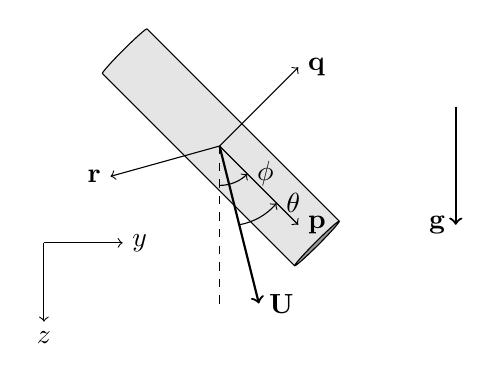
\begin{tikzpicture}[scale=1.]
%\node [rectangle, rotate=45, draw, minimum height=3cm, minimum width=1cm]  at (2, 2 ,2) (c) {}; %ne sera pas a lechelle mais pas grave
\node[cylinder, 
    draw = black, 
    text = black,
    cylinder uses custom fill, 
    cylinder body fill = black!10, 
    cylinder end fill = black!40,
    aspect = 0.2, 
    shape border rotate = 90, rotate =225, minimum height=3.5cm, minimum width=0.8cm] (c) at (2,2,2) {};

%\draw[ <->] (c.top)   -- (c.bottom) node [at end, left]   {$L$};
%\draw[ <->] (c.north) -- (c.south) node [at start, above] {$D$};

\draw[->] (2,2,2)   -- (3,1,2) node [at end, right]   {$\mathbf{p}$};
\draw[->] (2,2,2)   -- (3,3,2) node [at end, right]   {$\mathbf{q}$};
\draw[->] (2,2,2)   -- (1,2,3) node [at end, left]   {$\mathbf{r}$};

%\draw[->] (2.2,2,2) arc (-350:0:0.2);
%\draw[] (1.8,2.2,2) node[above]{$\mathbf{\Omega}$};
%\draw[] (2,2,2)  node []   {$\otimes $};%\mathbf{r}
%\draw[] (2,2,2)  node [above, left]   {$\mathbf{r}$};%

\draw[->, thick] (2,2,2)--(2.5,0,2) node[right]{$\mathbf{U}$};

\draw[-, dashed] (2,2,2)--(2,0,2);

\draw[->] (2.25,1,2) arc (-80:-40:0.8)node[right]{$\theta$};
\draw[->] (2,1.5,2) arc (-90:-45:0.5)node[right]{$\phi$};
%\draw (2.2,1.5,2) node[]{$\rho_p$};
\draw[->, thick] (5,2.5,2)--(5,1,2) node[left]{$\mathbf{g}$};

%\draw (0.5,1.5,2) node[]{$\rho_f, \mu$};

\draw[->] (-1,0,0)--(-1,-1,0)node[below]{$z$};
\draw[->] (-1,0,0)--(0,0,0)node[right]{$y$};

\end{tikzpicture}
\caption{Finite-length cylinder submitted to the gravity acceleration $\mathbf{g}$.}
\label{fig:single_cyl}
\end{figure}
We consider a finite-length cylinder of length $L$ and diameter $D$ settling under gravity with velocity $\mathbf{U}$ and angular velocity $\mathbf{\Omega}$ (Figure \ref{fig:single_cyl}). The main difficulty in studying this problem is the coupling between the body motion and the surrounding flow field which satisfies Navier-Stokes equations \citep{ern2012}.  The equations of motion expressed in a reference frame having its origin fixed with respect to the laboratory but axes rotating with the body read \citep{howe1995,mougin2002}

%The problem is governed by three dimensionless parameters. The Archimedes number $Ar$


%By making use of the  empirical formulas for the drag and torque, it is now possible to model accurately cylinders in a Lagrangian framework.
%Let's consider sedimenting cylinder in an inert fluid subject to buoyancy force only, besides, we only consider planar motion.
%Using Newton second law of motion we get,
%\begin{equation}
%    (m \delta_{ij}  + A_{ij}) \frac{d U_j}{dt}
%    +\epsilon_{ijk} \Omega_j (m\delta_{kl} + A_{kl})U_l
%    = F_i^{\omega}
%    + (m-\rho V)g_i,
%\end{equation}
%\begin{equation}
%    (I_{ij} + D_{ij})
%    \frac{d\Omega _j}{dt}
%    +\epsilon_{ijk} \Omega_j (I_{kl} + D_{kl})\Omega_l+\epsilon_{ijk} U_j A_{kl}U_l
%    = T_i^{\omega},
%\end{equation}
\begin{equation}
(m \mathbb{I} + \mathbb{A})\frac{\mathrm{d}\mathbf{U}}{\mathrm{d}t} + \boldsymbol{\Omega} \times ((m \mathbb{I} + \mathbb{A})\mathbf{U})  = \mathbf{F}^\omega+(m - \rho V) \mathbf{g},
\label{eq:forcebal}
\end{equation}

\begin{equation}
(\mathbb{J} + \mathbb{D})\frac{\mathrm{d}\boldsymbol{\Omega}}{\mathrm{d}t} + \boldsymbol{\Omega} \times ((\mathbb{J} + \mathbb{D})\boldsymbol{\Omega}) + \mathbf{U}\times (\mathbb{A}\times \mathbf{U})  = \mathbf{T}^\omega,
\label{eq:torquebal}
\end{equation}
where $m$ and $V$ are respectively the cylinder mass and volume, $\mathbb{I}$ is the identity matrix, $\mathbb{J}$ is the inertia tensor, $\mathbb{A}$ and $\mathbb{D}$ are the second-order added inertia tensors. Using indicial notation all those tensors, can be written as $J_{ij} = J_p p_ip_j+J_q(\delta_{ij}-p_ip_j)$, $A_{ij}= A_p p_ip_j+A_q(\delta_{ij}-p_ip_j)$ and $D_{ij} = D_q(\delta_{ij}-p_ip_j)$ where $\mathbf{p}$ is the unit orientation vector and $\mathbf{q}$ is the unit vector perpendicular to $\mathbf{p}$ in the plane $(y,z)$ (Figure \ref{fig:single_cyl}). If the components of the inertia tensor can be readily obtained in a closed form for a finite-length cylinder ($J_p = mD^2/8$, $J_q = m(3D^2/4+L^2)/12$) this is not the case for the components of the added mass tensors $A_p, A_q$ and $D_q$. If $A_p$ and $A_q$ have been already studied in the litterature \citep{loewenberg1993}, to the best of the author knowledge, no expression for $D_q$ has not been published yet. Based on the direct numerical simulation results of \citet{kharrouba2020} and the potential flow results of \citet{loewenberg1993} we derive correlations for $A_p$, $A_q$ and $D_q$ in Appendix \ref{app:added}. In equations \ref{eq:forcebal} and \ref{eq:torquebal}, $\mathbf{F}^{\omega}$ and $\mathbf{T}^{\omega}$ are the force and torque due to the vorticity in the flow. Except in inertia dominated regimes the motion of the cylinder is planar in the $(p,q)$ plane \citep{cabrera2022} and the equation of motion simplifies to  %Neglecting any angular motion 

%. Moreover $\Omega_p, \Omega_q = 0$. $\Omega = \Omega e_z$ and the equation of motion simplifies to 

\begin{align}
    (m + A_p) \frac{d U_p}{dt}
    - (m + A_q)\Omega _r U_q 
    &= F_p^{\omega}
    + (m-\rho V)g\cos \phi, \label{eq:Up}\\
    (m + A_q) \frac{d U_q}{dt}
    + (m + A_p)\Omega _r U_p 
    &= F_q^{\omega}
    - (m-\rho V)g\sin \phi,
\label{eq:Uq}\\
%\begin{equation}
    (J_{q} + D_{q})
    \frac{d\Omega _r}{dt}
    &= -U_pU_q(A_q-A_p) + T_r^{\omega}.
\label{eq:Omegar}
\end{align}
%\end{equation}

%We need to make dimensionless the previsous equation. On ne ne peut faire l'analyse dimensionel qu'en connaissant les regimes en Re. Non je ne pense pas. Si on dit que ce que l'on fait va jusqu'à des régimes modérement inertiel.
%Also, based on equation \ref{eq:torquebal} one may observe that a torque is already present in steady potential flow %for small but finite inertia effect and %For a sufficiently long cylindrical body in planar motion, this torque tends to align the sedimentation velocity to the minor axis of the body, as shown later in this section.
The physical origin of the torque can be exemplified by looking more closely at equation \ref{eq:Omegar}. In steady potential flow, a torque manifests on a cylindrical particle as indicated by the first term on the right-hand side of equation \ref{eq:Omegar} \citep{howe2006}. As the aspect ratio, $\chi = L/D$, exceeds 1, $A_q > A_p$ (see Appendix \ref{app:added}), and the torque is positive, orienting the body broad-side on.  As a result, to leading order the torque expression provided by \citet{khayat1989} for small Reynolds number and large aspect ratio ($\chi \gg 1$) $T_r = -5\pi/24\rho U_pU_qL^3/\ln ^2(\chi)$  is the sum of two positive contribution due to potential flow and vorticity. For $\chi \gg 1$ the potential contribution $-U_pU_q(A_q-A_p)$ scales as $-\rho \pi D^2U_pU_qL$ and is thus negligible to leading order in comparison to the vorticity contribution. The situation is less obvious for moderately large aspect ratio ($\chi \approx 2$) for which both contributions may have the same order of magnitude since the total torque on the body do not scales as $\rho U_pU_qL^3/\ln ^2(\chi)$ \citep{fintzi2023}. 

%The above set of equations are coupled to the Navier-Stokes equation which reads in a fixed reference frame as 




%This may have some important consequence in our problem for the neglect of the 

 %For spherical particles they were able to obtain a very interesting result:  the long-time decay of a particle suddenly set in motion from rest scales as $t^-2$ in the Oseen regime while it decays much slower in the Stokes regime as $t^{-1/2}$.


%Moreover non of the results initially obetained by lovalenti et brady do apply to the present configuration. Indeed the particle orientation change with time as well as the orientation of the velocity with respect to the particule orientation, this induced a drift of the particle position which may modify the results of Lovalenti due to the fact tthat the vorticity transportation in the cylinder wake is non-rectilinear.

%This slow time decay is characteristic of the Stokes flow regime. Indeed \citet{lovalenti1993}, have shown that the dacay of history force in the long time limit for a partcile accelrate suddnly form a fluid at rest is much faster. Also this decay seems to be very sensitive to the particular choice of kinematic choosen for the tparticle.


%for an impulsive start


%Moreover the quasi-steady counterpart of the fore 


%induce another inertial correction for a rotating and translating body.

%. This 

%Ce terme doit apparaitre pour le torque et les forces ? Regarding the hsitory force in the inertial regime very little work was dedicated to non-spherical particle. One may note the seminal work of Lovealenti et brady.
%translation and rotation


%Moreover there is no coupling between translation and rotation

%for a particle embedded in a uniform flow for
%In the limit of quasi-steady motion   

%as well as the coupling between rotation and translation when a non-spherical particle settles at finte Reynolds number \citet{cox1965}. In the limit of small inertia and particle ortating along their symmetry axis Cox was able to obtain the correction to rotating and accelerating cylinder.



%However one may do analytical progress in the limit of small but finite inertia,  In this limit, steady relative to some inertial frame of reference \footnote{Note that the results of Cox 1965, do not apply exactly to the present consifguration, since a the translating and rotating body cannot be written in a teady frame of reference. However one may expect the anayltical results of \citet{Cox1965} to be valid as long as the pseudo-inertial force are small}

%which can be written as $A_{ij}= \rho V (A_p^* p_ip_j+A_q^*(\delta_{ij}-p_ip_j))$ and $D_{ij} =\rho V L^2 D_q^*(\delta_{ij}-p_ip_j)$

% je pense qu'on peut discuter la limite des Re=0 puis celle des Re inertiels.



% je pense qu'il faut plutot analyser les points communs : a Re=0 pour des particules arbitraire (ou en tout cas des psheres ou cylindre), la decroissance se fait au temps long comme t^-1/2. En régimes d'Oseen pour toute particule decroissance 






%The assumption $\Omega L/U \ll 1$ will be discussed by comparing the results to published experimental work and direct numerical simulations in the next section. Under this assumption, the loads reduce to their quasi-steady counterpart (neglecting the $\Omega U$ contributions): $F_p^\omega \approx F_p$,  $F_q^\omega \approx F_q$ and -$U_pU_q(A_q-A_p) + T_r^{\omega} \approx T_r^i + T_r^\Omega$. $T_r^i$ is the inertial torque which makes the cylinder rotates toward its equilibrium position while $T_r^\Omega$ is the hydrodynamic torque resisting rotation. We will distinguish two different configurations depending on the cylinder aspect ratio: moderate aspect ratio $\chi \leq 30$ and long fibres $\chi > 30$. For $\chi \leq 30$ we will make use of the expression derived by \citep{kharrouba2021,pierson2021,fintzi2023} using slender-body theory and direct numerical simulations since they are more accurate than \citet{khayat1989} predictions. However, for $\chi > 30$ we will make use of \citet{khayat1989} expression.  To the best of the author's knowledge, finite-inertia effects have not been considered for a slender body rotating in a fluid at rest at infinity. Hence we will make use of the most accurate expression for this case under the Stokes flow assumption \citep{pierson2021}. The expression for $F_p$, $F_q$, $T_r^i$ and $T_r^\Omega$ are detailed in appendix \ref{app:qsloads}. In both cases, we make use of the linearized approximation to express the force as a function of the velocity of the particle. This approximation which is exact in the Stokes flow regime has proven to be accurate up to $Re \approx 1$ for $10 \leq\chi \leq 30$ and up to $Re_D \approx 10$ for $\chi < 10$\citet{fintzi2023}. Also, the experimental works of \citet{lopez2017} ($11.5 \leq \chi \leq 34.5$) and \cite{roy2019}  ($20 \leq \chi \leq 100$) have proven its relevance for larger aspect ratio.


%All the previous expressions are derived using slender-body theory and direct numerical simulations \citep{kharrouba2021,pierson2021,fintzi2023}. 

%As evidenced by  This simplied framework leads to a complex non-linear system of equations due to the  we assume a linearizd expression for the loads (as was done before by Roy et Lopez)

%in this paper are detailed in appendix \ref{app:qsloads}.

%n innovation they introduce
%is a linearized model in which the full equations of Khayat and Cox are used to
%predict drag forces on parallel and perpendicular fibres while the standard mobility
%tensor formalism is used to interpolate the forces for angles between these two limits.
%This greatly simplifies the calculation of drag forces since in general the nonlinear
%equations must be solved iteratively to find the particle velocity at which the drag
%force balances the applied force.


%Assuming therefore that
%the linear relation W i = M ij F j still holds with a modified mobility matrix that accounts for the

%This assumption can also be understood as the ratio between two time scales : 





%where closed form solutions based upon the analytical solution of 

%where analytical progress based on equation \ref{} and \ref{} and current knowledge of force and torque in moderaltey inertial regime. for  is possible for finite inertia effects and expression ... for the force torque. In particular since the expression fofr lift force ...
%To make some analytical progress one has too do assumption. As long as the rotation rate of the cylinder and its acceleration are small one may consider the problem as quasi-steady, and in this limit one mas neglect history term. 

%In the equation of fluid motion the unsteady term is much smaller than the inertial term as long as $\Omega L/ U$. 



%However we keep the inerttial term as weel as added mass effect, since they are the leading order term. + donne un indicateur de leur importnace. En fait dire que l'on néglige les effets d'hitoire car on néglige les temps courst c'est se tirer une balle dans le pied, car a ce moment la els effets ineritels type masse ajouté sont encore plus negligeables ? En gros on garde les temps courts mais on neglige les temps longs. Also we kept the particle inertia as well as added mass effect for three reasons. The first for the former is that it may become non-negligibel for sufficently high density ratio. Also we keep the added mass as the first effet of the fluid inertia on the body motion. Also when added mass effect will become important we will recall that the model will be probably false due to the neglect of the history force and coupling between rotation and tranlsation.

%$I_{ij} = I_p p_ip_j+I_q(\delta_{ij}-p_ip_j)$ is the inertia tensor, $A_{ij}= \rho V (A_p p_ip_j+A_q(\delta_{ij}-p_ip_j))$ and $D_{ij} =D_p p_ip_j+D_q(\delta_{ij}-p_ip_j)$ are the second-order added inertia tensors. 

%If $I_p = m/8D^2$ and $I_q= m/12(3/4D^2+L^2)$ can be readily obtained in a closed form for a finite-length cylinder this is not the case for $A_p$, $A_q$ and $D_q$ ($D_p = 0$ since the rotation of a cylinder along its own axis do not generate any momentum in potential flow).



\section{Short-time dynamics}

\label{sec:short}
In the high-frequency limit or equivalently for time shorter than the diffusive scale added mass effect dominates over viscous contribution. This may be proved by deriving the unsteady loads in the Stokes regime \citet{kabarowski2020}, but also by performing a short time-analysis of the Navier-Stokes equation \citet{mougin2002}. The latter is more general as it is not limited to the Stokes flow regime. The proper length scale to be used in the diffusive scale for the problem at hand is unknown \textit{a priori}. However, \citet{kabarowski2020} have shown that for both transverse and longitudinal oscillations, the added mass contributions dominate over the history load if $t \ll D^2 /\nu$. Hence, the proper length scale in the short dynamic is the cylinder diameter, at least in the Stokes flow regime. Assuming $t \ll D^2 /\nu$, equations \ref{eq:Up} - \ref{eq:Omegar} simplify to


%For the problem of interest, the proper length scale to be used in the diffusive scale is \textit{a priori} unknown. However, \citet{kabarowski2020} have shown for both transverse and longitudinal oscillation the added mass contributions dominate over history load if $t \ll D^2 /\nu$. Hence the proper length scale in the short dynamic is the cylinder diameter at least in the Stokes flow regime. Assuming $t \ll D^2 /\nu$ equations \ref{eq:Up}, \ref{eq:Uq} and \ref{eq:Omegar} reduce to
%related to the diffusive scale is a priori unknown since the cylinder is characterized by two length scale. 

%all manifestation of the vorticity are negligible \citet{mougin2001}.

%($t\ll a^2/\nu$), all manifestation of the vorticity are negligible. (a verifier plus prorement dans le bouquin de papier de Jacques) This may be prooved (I guess), by the short time analysis perfomed by \citet{mougin2001}, and also since in the fourier space the high frequency limit is dominated by added mass effect

% the above equations reduce to :

\begin{align}
    (m + A_p) \frac{d U_p}{dt}
    - (m + A_q)\Omega _r U_q 
    &= (m-\rho V)g\cos \phi, \label{eq:Upv}\\
    (m + A_q) \frac{d U_q}{dt}
    + (m + A_p)\Omega _r U_p 
    &= - (m-\rho V)g\sin \phi,
\label{eq:Uqv}\\
%\begin{equation}
    (J_{q} + D_{q})
    \frac{d\Omega _r}{dt}
    &= -U_pU_q(A_q-A_p) ,
\label{eq:Omegarv}\\
\frac{d \phi}{dt} &=\Omega _r \label{eq:Phiv},
\end{align}
where we made explicit the equation ruling the dependency of $\phi$ with time. To the best of our knowledge, there is no closed form analytical solution to this non-linearly coupled system of equations, although there is a straightforward analytical treatment in the case of zero gravity \citet{lamb1953}. We have to solve this system numerically but one may get insightful estimates using asymptotic analysis. By balancing the acceleration of gravity with the particle acceleration in equations \ref{eq:Upv} and \ref{eq:Uqv} one get $U \sim gT$ where $U$ is a characteristic velocity scale, and $T$ a characteristic timescale. Injecting this scaling in equation \ref{eq:Omegarv}, and since $(A_q-A_p) / (I_{q} + D_{q}) \sim 1 /L^2$ for $\chi \gg 1$  one get the characteristic angular velocity $\Omega \sim g^2T^3/L^2$. By using this estimates in equations \ref{eq:Upv}, \ref{eq:Uqv}, \ref{eq:Omegarv} and \ref{eq:Phiv} and defining the dimensionless (starred) quantities as $U_p = U U_p^*$, $U_q = U U_q^*$ and $\Omega_r = \Omega ^*\Omega_r$ we obtain

%To the best of our knowledge there is no analytical solution to this non-linearly coupled systeme of equations (also there is a straightfoward analytical treatement in the case of zero force see Lamb art 127) Beside of solving it numerically one may get insight using asymptotic estimates. 
%We assume that the coupling term in 6 et 7 are neglgiiglbe at leading order. this may be justified a posteriori using scaling analysis. By balancing particle inertia with the history force one get $ U_p \sim g T$ and $U_q \sim g T$. Injecting the previsous scaling in the angular momentum equation one obtain $\Omega _r \sim g^2T^3/L^2$. Hence $\Omega_r U_p \sim g^3T^4/L^2$. Hence as long as $T \ll (L/g)^0.5$ the coupling term a negligible. In mayny pratical configuration of interest this condition is met. If we assume that there is no coupling term  

%made of equations \ref{eq:Up}, \ref{eq:Uq} and \ref{eq:Omegar} with the absence of vorticity contributions.

%Neglecting the vorticity contributions in equations \ref{eq:Up}, \ref{eq:Uq} and balancing the acceleration of gravity with the particle acceleration one get $U \sim gT$, where $U$ is the characteristic velocity, and $T$ a characteristic timescale. Injecting this scaling in equation \ref{eq:Omegar} and still neglecting the contribution of the vorticity, one get the characteristic angular velocity $\Omega \sim g^2T^3/L^2$

%From 6 and 7 one get a natural scaling for the acceleration $U_p/T \sim g$  


%Attention il faut uniformiser les notations pour les coefficients de masse ajoute que tout soit bien homogène.

\begin{align}
 \frac{d U_p ^*}{dt^*}
    - \epsilon \frac{\mathcal{A}}{\mathcal{B}}\Omega _r ^* U_q ^* 
    &= \mathcal{A}\cos \phi, \label{eq:Upvd}\\
    \frac{d U_q ^*}{dt^*}
    + \epsilon\frac{\mathcal{B}}{\mathcal{A}}\Omega _r ^* U_p ^* 
    &= -\mathcal{B}\sin \phi, \label{eq:Uqvd}\\
%\begin{equation}
    \frac{d\Omega _r^*}{dt^*}
    &= -\mathcal{C}U_p^*U_q^* ,
\label{eq:Omegarvd}\\
\frac{d \phi}{dt^*} &=\epsilon\Omega _r^* \label{eq:Phivd},
\end{align}
where $\mathcal{A}=(\bar{\rho}-1)/(\bar{\rho}+A_p^*)$, $\mathcal{B}=(\bar{\rho}-1)/(\bar{\rho}+A_q^*)$, $\mathcal{C}=(A_q^*-A_p^*)/(\bar{\rho}J_q^*+D_q^*)$, $A_p^* = A_p / (\rho V), A_q^*= A_q / (\rho V)$, $J_q^* = J_q/ (\rho VL^2)$, $D_q^* = D_q/ (\rho VL^2)$, $\bar{\rho}=\rho _p/\rho$ is the density ratio and $\epsilon = g^2T^4/L^2$ can be understood as the ratio of the characteristic timescale over a gravity time scale. In the following, we consider the small time limit $T \ll (L/g)^{1/2}$   or equivalently $\epsilon \ll 1$. We seek for solutions of equations \ref{eq:Upvd} - \ref{eq:Phivd} in the form of asymptotic expansions in powers of the small parameter $U_p^* = U_p^{*(0)}+\epsilon U_p^{*(1)}+...$, $U_q^* = U_q^{*(0)}+\epsilon U_q^{*(1)}+...$, $\Omega _r^* = \Omega _r^{*(0)}+\epsilon \Omega_r^{*(1)}+...$ and $\phi = \phi^{(0)}+\epsilon \phi^{(1)}+...$. The calculations are straightforward and are detailed in appendix \ref{app:short}. The solutions up to the order 1 with respect to the small parameter $\epsilon$ are 

\begin{align}
U_p ^{*} &=   \mathcal{A}t^*\cos \phi^{(0)} -\frac{\epsilon}{12}\mathcal{A}^2\mathcal{B}\mathcal{C}t^{*5}\cos \phi^{(0)} \sin ^2\phi^{(0)}+\mathcal{O}(\epsilon ^2) \label{eq:upt}, \\
U_q ^{*} &=   -\mathcal{B}t^*\sin \phi^{(0)}-\frac{\epsilon}{12}\mathcal{A}\mathcal{B}^2\mathcal{C}t^{*5}\cos ^2\phi^{(0)} \sin \phi^{(0)}+\mathcal{O}(\epsilon ^2) \label{eq:uqt},\\
\Omega _r^{*} &= \frac{\mathcal{A}\mathcal{B}\mathcal{C}}{3}t^{*3}\cos \phi^{(0)} \sin \phi^{(0)}+\mathcal{O}(\epsilon ^2),\\
\phi^{}&=\phi^{(0)} + \epsilon\frac{\mathcal{A}\mathcal{B}\mathcal{C}}{12}t^{*4}\cos \phi^{(0)} \sin \phi^{(0)} +\mathcal{O}(\epsilon ^2).
\end{align} 


%we compute the first correction due to the non-linear coupling between all the equations. 
%Hence one may find a regular perturbation solution to this problem by looking a perturbation sery as 



%In this limit ... the $\Omega _r ^* U_q ^*$ and $\Omega _r ^* U_p ^*$  are negligible provided that $\epsilon = \frac{g^2T^4}{L^2} \ll 1$ or equivalently $T \ll (L/g)^{1/2}$. Moreover under the same condition the variation of the angle $\phi$ with time is negligible. 

\begin{figure}[h!]
    \centering
        \includegraphics[height=0.23\textwidth]{U_p_t}
        \includegraphics[height=0.23\textwidth]{U_q_t}
        \includegraphics[height=0.23\textwidth]{Omega_t}\\
        \vspace{-3mm}
        \hspace{0cm}(a) \hspace{5cm} (b) \hspace{5cm} (c)\\
        \includegraphics[height=0.23\textwidth]{U_p_t_10}
        \includegraphics[height=0.23\textwidth]{U_q_t_10}
        \includegraphics[height=0.23\textwidth]{Omega_t_10}\\
        \vspace{-3mm}
        \hspace{0cm}(d) \hspace{5cm} (e) \hspace{5cm} (f)\\
        \includegraphics[height=0.23\textwidth]{U_p_t_1000}
        \includegraphics[height=0.23\textwidth]{U_q_t_1000}
        \includegraphics[height=0.23\textwidth]{Omega_t_1000}\\
        \vspace{-3mm}
        \hspace{0cm}(g) \hspace{5cm} (h) \hspace{5cm} (i)\\
    \caption{Dimensionless velocities and angular velocity as function of time for a $\chi=10$ cylinder starting from rest with $\phi=30^\circ$ and $\epsilon = 1$. (a), (b), (c) : $\bar{\rho} = 1.5$. (d), (e), (f) : $\bar{\rho} = 10$. (g), (h), (i) : $\bar{\rho} = 1000$. $-$ : numerical solution of equations \ref{eq:Upvd}, \ref{eq:Uqvd}, \ref{eq:Omegarvd} and \ref{eq:Phivd}, $--$ : zero-th order asymptotic expansion, $-\cdot-$ : first order asymptotic expansion.}
    \label{fig:short}
\end{figure}
Figure \ref{fig:short} displays the numerical and analytical solutions for a cylinder of aspect ratio $10$ released with an orientation angle $\phi =30 ^\circ$. We impose $\epsilon = 1$ such that $T = (L/g)^{1/2}$. The numerical solution is obtained by using a Runge-Kutta 4 algorithm. For $\bar{\rho} =1.5$ a good agreement is observed between the numerical and solution and the zeroth order analytical solution up to $t^* \approx 1.5$ and up to $t^*  \approx2.5$ for the first order solution (Figures \ref{fig:short} (a), (b) and (c)). For moderately large density ratios the agreement with the numerical solution is slightly worse. However, for the largest density ratios the first-order analytical solutions remain valid up to $t^*\approx 6$ (Figures \ref{fig:short} (g), (h) and (i)). For all the density ratios one may observe the good agreement between the analytical and numerical solutions out of the range of applicability of the analytical solution. Also, this agreement seems to be dependent on $\bar{\rho}$. The explanation lies in the magnitude of the coupling terms between translation and rotation in equations \ref{eq:Upvd} and \ref{eq:Uqvd}. At first-order this coupling terms are found to be proportional to $\mathcal{A}^2\mathcal{B}\mathcal{C}$ and $\mathcal{A}\mathcal{B}^2\mathcal{C}$ in equations \ref{eq:upt} and \ref{eq:uqt}. 


%From these results, a natural question arises: why is the agreement with the numerical solution so good while the asymptotic analysis is performed under the assumption $t^* \ll 1$ for $\epsilon = 1$? The explanation lies in the magnitude of the coupling terms between translation and rotation in equations \ref{eq:Upvd} and \ref{eq:Uqvd}. At first-order this coupling term are found to be proportional to $\mathcal{A}^2\mathcal{B}\mathcal{C}$ and $\mathcal{A}\mathcal{B}^2\mathcal{C}$ in equations \ref{eq:upt} and \ref{eq:uqt}. 

%One can observe that the magnitude of the coupling term $\Omega _r ^* U_q ^*$ and $\cos \phi$ at  first order are proportionnal to $\mathcal{A}^2\mathcal{B}\mathcal{C}$ and $\mathcal{A}\mathcal{B}^2\mathcal{C}$. Hence a simple way to evaluate the magnitude of this term is.

%In practice, one may anticipate that the range of validity of the analytical solution may be also dependent of the dimensionless parameters $\bar{\rho}$ and $\chi$. 

%is very dependent on the value of the magnitude of the coupling term, which of course depends at leading order of $\epsilon$ but also of $\mathcal{A}^2\mathcal{B}\mathcal{C}$


%Also the range of validity of the analytical solution is very dependent on the value of the magnitude of the coupling term, which of course depends at leading order of $\epsilon$ but also of $\mathcal{A}^2\mathcal{B}\mathcal{C}$.

\begin{figure}[h!]
    \centering
        \includegraphics[height=0.26\textwidth]{A2BC}
        \includegraphics[height=0.26\textwidth]{AB2C}
    \caption{Leading order terms coupling translation and rotation. $-$ : $\chi =2$, $--$ : $\chi =8$, $-\cdot-$ : $\chi =32$, $\cdot \cdot \cdot$ : $\chi \rightarrow \infty$.}
    \label{fig:ABC}
\end{figure}
Figure \ref{fig:ABC} illustrates the variation of $\mathcal{A}^2\mathcal{B}\mathcal{C}$ and $\mathcal{A}\mathcal{B}^2\mathcal{C}$ as a function of $\chi$ and $\bar{\rho}$. Both coupling terms have the same order of magnitude and are smaller than approximatively $0.8$. The behaviour of $\mathcal{A}^2\mathcal{B}\mathcal{C}$ and $\mathcal{A}\mathcal{B}^2\mathcal{C}$ as function of $\chi$ and $\bar{\rho}$ disserve also some comments. Since both quantity evolves comparably, we will focus on $\mathcal{A}^2\mathcal{B}\mathcal{C}$. This quantity increases as a function of $\chi$ for moderate $\chi$. Hence one may expect a better match of the theory for small cylinders. Then $\mathcal{A}^2\mathcal{B}\mathcal{C}$ becomes nearly independent of $\chi$  for $\chi \approx 20$. This is in line with the results of appendix \ref{app:added} in which the added mass coefficients become almost independent of $\chi$ for this aspect ratio. $\mathcal{A}^2\mathcal{B}\mathcal{C}$ behaves non-monotonously with $\bar{\rho}$. It increases for $\bar{\rho} \leq 5$ and then decreases for larger $\bar{\rho}$. The value of $\bar{\rho}$ for which we observed the maxima is weakly dependent on $\chi$. All these trends can be easily obtained by looking more closely at the behaviour of  $\mathcal{A}^2\mathcal{B}\mathcal{C}$ as a function of $\bar{\rho}$. First one may note that for $\bar{\rho}\rightarrow 1$ we have $\mathcal{A}^2\mathcal{B}\mathcal{C} \sim (\bar{\rho} - 1) ^3(A_q^*-A_p^*)/[(1+A_p^*)^2(1+A_q^*)(J_q^*+D_p^*)]$ which explains the strong increase of $\mathcal{A}^2\mathcal{B}\mathcal{C}$ for $\bar{\rho} \leq 5$. In the opposite limit $\bar{\rho} \gg 1$ one obtain $\mathcal{A}^2\mathcal{B}\mathcal{C} \sim 1/ \bar{\rho}\times(A_q^*-A_p^*)/J_q^*$ which explains the decay of $\mathcal{A}^2\mathcal{B}\mathcal{C}$ for large density ratio. 

%Moreover a rough estimate of the value of $\bar{\rho}$ for which we observed the maxima can be obtained by matching the two previous $\mathcal{A}^2\mathcal{B}\mathcal{C}$ estimates.  The extremum is obtained for value of $\bar{\rho}$ following $(\bar{\rho} - 1) ^3\bar{\rho} \sim (1+A_p^*)^2(1+A_q^*)(J_q^*+D_p^*)/J_q^*$. For  $\chi \gg 1$, $A_p^* = 0$, $A_q^* = 1$, $J_q^*=1/12$ and $D_q^* =1/12$ and one obtain $(\bar{\rho} - 1) ^3\bar{\rho} \sim 4$ which leads to $\bar{\rho} \approx 2.22$ a value not so far from the numerically obtained one ($\bar{\rho} \approx 3$).

%Hence the first order correction in equations \ref{eq:Upvd} and \ref{eq:Uqvd} is even smaller than $\epsilon$. This is the main reason which explains the good agreement between the analytical and numerical solutions out of the range of applicability of the analytical solution.

%$\mathcal{A}^2\mathcal{B}\mathcal{C} \sim (\bar{\rho} - 1) ^3(A_q^*-A_p^*)/[(1+A_p^*)^2(1+A_q^*)(J_q^*+D_p^*)]$


%In the configuration of a particle settling under gravity from rest the solution in diamensional form reads :


It is also interesting to discuss the range of applicability of the asymptotic results in experiments. Our observations suggest that the asymptotic expansion is valid up to $t \sim (L/g)^{1/2}$ and even larger value for large density ratios. Thus one may expect this solution to be valid as long as $(L/g)^{1/2} \ll D^2 /\nu$ which can be written $Ar \gg (\bar{\rho}-1)\chi$ where $Ar = (\rho _p -\rho)\rho g D^3/\mu^2$ is the Archimedes number. This implies that for sufficiently inertial regimes, the proposed analytical solution is expected to be observed in experiments. We are not aware of any experiments specifically dedicated to testing the validity of the theory. However, the qualitative observations provided in \citet{toupoint2019} may provide a first comparison with the present results. \citet{toupoint2019} investigated the settling of cylinder in inertia dominated regime $Ar \approx 40000$. Their density ratio was fixed to $\bar{\rho} = 1.16$ and the elongation ratio of the cylinders ranged between $2$ and $20$. In particular, the time related to viscous diffusion in their experiments with a cylinder of diameter $2$mm and $\chi =5$ is $t_\nu \approx 4s$ while $T \approx 0.03s$.  Hence the present theory should apply to their experimental results. They observed that the distance needed for the cylinders to rotate to their equilibrium position was less than $10d$ even when the cylinder was released vertically. From our analytical results, we obtain the time needed for the cylinder to change its orientation from nearly vertical ($\phi^{(0)} \ll 1$) to horizontal ($\phi(t^*) = \pi/2$) $t \sim (L/g)^{1/2} (6\pi/(\phi^{(0)}\mathcal{A}\mathcal{B}\mathcal{C}))^{1/4}$. With $\phi^{(0)} = \pi/10$ one get $t \approx 0.2s$. Injecting this estimate in the velocity equation and integrating one obtains the normalised distance $l/D$ for which the cylinder changes its orientation: $l/D = \mathcal{A}gt^2/2 \approx 11.2$. This estimate is very close to the experimental prediction and gives confidence on the non-viscous flow origin on which this model is grounded.





%(redefinir le nombre d'Archimede avec la definition de la section suivante)



%\section{Quasi-steady regime : scaling analysis}
\section{Quasi-steady models}
%\section{Long-time dynamic}
\label{sec:scaling}

The particle equations of motion (\ref{eq:Up} - \ref{eq:Omegar}) are coupled to the Navier-Stokes equations \textit{via} the boundary conditions and the hydrodynamic loads. This make the problem very hard to solve and simplifying assumptions are required to make analytical progress as explained in the introduction. Since the characteristic time needed for the body to change its orientation scales like $\Omega ^{-1}$, the unsteady term in the Navier-Stokes equation scales as $\rho U \Omega$ where $\Omega$ and $U$ may be taken as the nominal scales for the angular and settling velocities. Since the inertial term scales as $\rho U^2 / L$ the unsteady term is negligible in comparison to the inertial term as long as $\Omega L /U \ll 1$. This condition is satisfied when the time needed for the vorticity to diffuse from the body for a Reynolds number of unity is much smaller than the rotation time scale \citep{newsom1994}. In this limit, one may consider the fluid unsteady term and as a consequence the history loads to be negligible. To be fully consistent with the neglect of the unsteady term we will also neglect the added mass loads. It remains to consider the inertial correction to the loads proportional to $\Omega U$. One may expect the $\Omega U$ corrections to be smaller than the inertial $U^2$ corrections as long as $\Omega L/U \ll 1$. Hence under the assumption, we postulate that both the history terms and the $\Omega U$ contribution are negligible with respect to the other load contribution as long as $\Omega L/U \ll 1$. The choice of the length of the particles ensures that the particle length is the relevant scale in the limit of a slender fibre \citep{khayat1989,dabade2015}. %Also, this choice may be 
The validity of the assumption $\Omega L/U \ll 1$ will be evaluated through comparisons with experimental results and direct numerical simulations in Section \ref{sec:exp_dns}. 


%Based on scaling arguments \citet{pierson2021} have shown that this assumption remains valid during sedimentation as long as inertia is negligible in comparison to viscous effect.

%In this part we investigate the long-time behaviour of equations \ref{eq:Up}, \ref{eq:Uq} and \ref{eq:Omegar}. We assume that $\Omega L/ U \ll 1$ such that both the history terms and $\Omega U$ load contribution may be neglected. 

\subsection{Quasi-steady models for an arbitrarily oriented cylinder}

Under the assumption $\Omega L/U \ll 1$, the loads can be approximated as their quasi-steady counterparts, disregarding the $\Omega U$ terms: $F_p^\omega \approx F_p$, $F_q^\omega \approx F_q$ and $-U_pU_q(A_q-A_p) + T_r^{\omega} \approx T_r^i + T_r^\Omega$ where $F_p$ and $F_q$ are the quasi-steady forces in the longitudinal and perpendicular directions to the cylinder. The inertial torque, $T_r^i$, drives the cylinder towards its equilibrium position, while the hydrodynamic torque, $T_r^\Omega$, resists rotation. We will distinguish two different configurations depending on the cylinder aspect ratio: moderately long rods $ 2\leq \chi \leq 30$ and long fibres $\chi > 30$. For $\chi \leq 30$, expressions derived through slender-body theory and direct numerical simulations by \citet{kharrouba2021,pierson2021,fintzi2023} will be used, as they provide more accurate predictions compared to those by \citet{khayat1989}. Conversely, the expression by \citet{khayat1989} will be used for $\chi > 30$. To the author's knowledge, finite-inertia effects have not been considered for a slender body rotating in a fluid at rest at infinity. Thus, the most accurate expression for this case under the Stokes flow assumption by \citet{pierson2021} will be used. The expressions for $F_p$, $F_q$, $T_r^i$, and $T_r^\Omega$ are outlined in Appendix \ref{app:qsloads}. In both configurations, the linearized approximation is employed to describe the force as a function of the particle velocity. This approximation, which is exact in the Stokes flow regime, has been demonstrated to be accurate up to $Re \approx 1$ for $10 \leq\chi \leq 30$ and up to $Re \approx 10$ for $\chi < 10$ by \citet{fintzi2023} where $Re = \rho D U/\mu$ is the Reynolds number based on the body diameter. The experimental works of \citet{lopez2017} with $11.5 \leq \chi \leq 34.5$ and \citet{roy2019} with $20 \leq \chi \leq 100$ have also validated its relevance for larger aspect ratios.


%The Stokes flow assumption will be validated \textit{a posteriori}.

%\color{red}
%ajouter la dependance en theta pour le torque dans le cas general.
%\color{black}

%for small but finite Reynolds number based on the body diameter $Re = \rho U D /\mu$.


%validity of the so-called quasi-steady assumption. %Au sens de Cox cela signifie que $dU/dt$ et $\Omega$ sont petit devant 1. De plus nous supposons que le termer en $\Omega U$ est faible.

%\subsection{Low Archimedes number : $Ar \ll 1$}

%\subsection{Scaling analysis}


%\subsubsection{$\chi \sim \mathcal{O}(1)$}
Equations \ref{eq:Up} - \ref{eq:Omegar} are normalized by defining dimensionless (starred) quantities as $U_p = U U_p^*$, $U_q = U U_q^*$, $\Omega_r = \Omega \Omega ^*$ and $t = \Omega ^{-1}t^*$ where the characteristic angular and velocity scales are \textit{a priori} unknown. In the small inertia limit making use of the linearized approximation, the forces can be expressed as $F_p = -\mu U U_p^* L F_p^*(Re_L^*,\chi) $ and $F_q = -\mu U U_q^*L F_q^*(Re_L^*,\chi) $ where the expressions for $F_p$ and $F_q$ can be obtained from appendix \ref{app:qsloads}. $Re_L^* = Re_L(U_p^{*2}+U_q^{*2})^{1/2}$ is the Reynolds number based on the instantaneous settling velocity while $Re_L = \rho U L/(2\mu)$ is the characteristic Reynolds number based on the body half length. The inertial torque reads $ -\rho U^2U_p^*U_q^* L^3T_i^*(Re_L^*,\chi, \theta)$ while the torque resisting rotation reads $-\mu \Omega \Omega _r^* L^3 T_\Omega^*(Re_\Omega ^*,\chi)$ where $Re_\Omega^* = Re_\Omega|\Omega_r^*|$ and $Re_\Omega = \rho \Omega D^2/\mu$. Injecting all those scaling in equations \ref{eq:Up}, \ref{eq:Uq} and \ref{eq:Omegar} one obtain

%\begin{align}
%    Re_\Omega\left[\left(\bar{\rho}+A_p^*\right)\frac{d U_p^*}{dt^*}
%    - \left(\bar{\rho}+A_q^*\right)\Omega_r^* U_q^* \right]
%    &= -\frac{4}{\pi}F_p^*(Re_L^*,\chi) U_p^*
%    + \frac{(\rho _p-\rho)gD^2}{\mu U}\cos \phi, \label{eq:Up*}\\
%    Re_\Omega\left[\left(\bar{\rho}+A_q^*\right)\frac{d U_q^*}{dt^*}
%    + \left(\bar{\rho}+A_p^*\right)\Omega_r^* U_p^* \right]
%    &= -\frac{4}{\pi}F_q^*(Re_L^*,\chi) U_q^*
%    - \frac{(\rho _p-\rho)gD^2}{\mu U}\sin \phi, 
%\label{eq:Uq*}\\
%  (\bar{\rho}J_q^* + D_{q}^*)\left(\frac{Re_\Omega}{Re}\right)^2
%    \frac{d\Omega _r ^*}{dt ^*}
%    &= -\frac{4}{\pi}\left(T_i^*(Re_L^*,\chi, \theta)U_p^*U_q^* + \frac{\mu \Omega }{\rho U^2}T_\Omega^*(Re_\Omega ^*,\chi)\Omega _r^*\right).
%\label{eq:Omegar*}
%\end{align}
\begin{align}
    \bar{\rho} Re_\Omega  \left(\frac{d U_p^*}{dt^*}
    - \Omega_r^* U_q^* \right)
    &= -\frac{4}{\pi}F_p^*(Re_L^*,\chi) U_p^*
    + \frac{(\rho _p-\rho)gD^2}{\mu U}\cos \phi, \label{eq:Up*}\\
    \bar{\rho} Re_\Omega \left(\frac{d U_q^*}{dt^*}
    + \Omega_r^* U_p^* \right)
    &= -\frac{4}{\pi}F_q^*(Re_L^*,\chi) U_q^*
    - \frac{(\rho _p-\rho)gD^2}{\mu U}\sin \phi, 
\label{eq:Uq*}\\
  \bar{\rho}\left(\frac{Re_\Omega}{Re}\right)^2 J_q^*
    \frac{d\Omega _r ^*}{dt ^*}
    &= -\frac{4}{\pi}\left(T_i^*(Re_L^*,\chi, \theta)U_p^*U_q^* + \frac{\mu \Omega }{\rho U^2}T_\Omega^*(Re_\Omega ^*,\chi)\Omega _r^*\right).
\label{eq:Omegar*}
\end{align}


From the above set of equations and for moderate density ratios $\bar{\rho} \sim 1$ it appears that all the unsteady terms vanish if $Re_\Omega \ll 1$ and $Re_\Omega \ll Re$. In contrast for large density ratios, one may take into account the particle inertia \citep{newsom1994}. We have to recall that to derive equations \ref{eq:Up*} - \ref{eq:Omegar*}  we have to assume $\Omega L /U \ll 1$, which is equivalent to $Re_\Omega \ll \chi Re$. This a rather restrictive condition for the applicability of the model but we shall see hereafter that it is valid for a non-negligible range of dimensionless parameters. Since the last terms in equation \ref{eq:Up*} - \ref{eq:Omegar*} must be of order one the velocity and angular velocity scales can be readily obtained as $U\sim D^2(\rho _p-\rho)g/\mu$ and $\Omega = \rho D^4(\rho _p-\rho)^2g^2/\mu^3$. Inserting these scalings yields


%Balancing the weight of the cylindrical particles with the hydrodynamic forces gives the characteristic velocity $U\sim D^2(\rho _p-\rho)g/\mu$. It remains to obtain the characteristic angular velocity. The inertial torque reads $ -\rho U^2U_p^*U_q^* L^3T_i^*(Re_L,\chi) $ with the torque resisting rotation which reads $-\mu \Omega \Omega _r^* L^3 T_\Omega^*(Re_\Omega,\chi)$ with $Re_\Omega = \rho \vert\boldsymbol{\Omega }LD/(2\mu)\vert$. Balancing both torques together one obtain $\Omega \sim \rho U^2/\mu$ and finally $\Omega = \rho D^4(\rho _p-\rho)^2g^2/\mu^3$. Injecting all those scaling in equations Equations \ref{eq:Up}, \ref{eq:Uq} and \ref{eq:Omegar} one obtain

  %contribution to the loads under the assumption ... Using the former scaling this asumption can be written ... we will discuss this in the 


%The last assumption is retaher restrictive since the angular veloicity must 

%(as well as the omega u coupling terms). 




%In the limit of negligible inertia the equation of motion are linear the forces are made dimensionless as follow $F_p = \mu U L F_p^*(\chi,Re_L) \cos\theta$ and  . Balancing the weight with the drag force gives the charcateristic velocity $U\sim D^2(\rho _p-\rho)g/\mu$ 

%(dans les faits ce "balance" ne semble pas trop mauvais pour tous les chi, car seul $F_p$ ne suit pas cette loi pour les bas chi, donc a mon avis c'est le "meilleur balance" possible à ce stade). Si l'on divise l'équation précédente par la flottabilite on a 
%\begin{equation}
%    \frac{\rho _p +\rho  A_p}{\rho _p -\rho} \frac{U}{Tg}\frac{d U_p^*}{dt^*}
%    - \frac{\rho _p +\rho  A_q}{\rho _p -\rho} \frac{U \Omega}{g}\Omega^* U_q^* 
%    = F_p^{\omega}*\frac{\mu U L }{(\rho _p -\rho)V_pg}
%    + \cos \phi
%\end{equation}
%Puisque $U\sim D^2(\rho _p-\rho)g/\mu$
%\begin{equation}
%    \frac{\rho\Omega D^2}{\mu}\left[\left(\frac{\rho _p}{\rho}+A_p\right)\frac{d U_p^*}{dt^*}
%    - \left(\frac{\rho _p}{\rho}+A_q\right)\Omega^* U_q^* \right]
%    = \frac{4}{\pi}F_p^*(Re_L,\chi) \cos \theta
%    + \cos \phi
%\end{equation}

%\begin{align}
%    Ar^2\left[\left(\bar{\rho}+A_p^*\right)\frac{d U_p^*}{dt^*}
%    - \left(\bar{\rho}+A_q^*\right)\Omega_r^* U_q^* \right]
%    &= -\frac{4}{\pi}F_p^*(Re_L^*,\chi) U_p^*
%    + \cos \phi, \label{eq:UpA**}\\
%    Ar^2\left[\left(\bar{\rho}+A_q^*\right)\frac{d U_q^*}{dt^*}
%    + \left(\bar{\rho}+A_p^*\right)\Omega_r^* U_p^* \right]
%    &= -\frac{4}{\pi}F_q^*(Re_L^*,\chi) U_q^*
%    - \sin \phi, 
%\label{eq:UqA**}\\
%    Ar^2 (\bar{\rho}J_q^* + D_{q}^*)
%    \frac{d\Omega _r ^*}{dt ^*}
%    &= -\frac{4}{\pi}\left(T_i^*(Re_L^*,\chi, \theta)U_p^*U_q^* + T_\Omega^*(Re_\Omega^*,\chi)\Omega _r^*\right).
%\label{eq:OmegarA**}
%\end{align}


\begin{align}
    \bar{\rho} Ar^2  \left(\frac{d U_p^*}{dt^*}
    - \Omega_r^* U_q^* \right)
    &= -\frac{4}{\pi}F_p^*(Re_L^*,\chi) U_p^*
    + \cos \phi, \label{eq:UpA**}\\
    \bar{\rho} Ar^2 \left(\frac{d U_q^*}{dt^*}
    + \Omega_r^* U_p^* \right)
    &= -\frac{4}{\pi}F_q^*(Re_L^*,\chi) U_q^*
    - \sin \phi, 
\label{eq:UqA**}\\
  \bar{\rho}Ar^2 J_q^*
    \frac{d\Omega _r ^*}{dt ^*}
    &= -\frac{4}{\pi}\left(T_i^*(Re_L^*,\chi, \theta)U_p^*U_q^* + T_\Omega^*(Re_\Omega^*,\chi)\Omega _r^*\right).
\label{eq:OmegarA**}
\end{align}


The dimensionless nonlinear system of coupled differential equations, represented by Equations \ref{eq:UpA**} - \ref{eq:OmegarA**}, describe the velocity and angular velocity of a cylinder under an external force. Analytical solutions to this system can only be obtained in the limit of low Archimedes number, as reported by \citet{cox1965}. Otherwise, numerical solutions must be sought. Note that $\bar{\rho} Ar^2$ can be seen as a Stokes number ($St$) which is a dimensionless measure of particle inertia. The system exhibits two distinct regimes depending on $St$. For moderate particle inertia ($St \sim 1$ or equivalently $\bar{\rho}\sim 1/Ar^2$), as in the case of small solid particles settling in air, the left-hand sides (LHS) of equations \ref{eq:UpA**} - \ref{eq:OmegarA**} are non-negligible. The resulting system then consists of three ordinary differential equations which are solved thanks to a Runge-Kutta 4 algorithm.  Conversely, for small particle inertia ($St \ll 1$) as for small particles with densities close to that of the fluid the 
(LHS) can be neglected. The simplified system is a non-linear function composed of three equations, which can be solved using classical root finding methods. It reads 
\begin{align}
0
    &= -\frac{4}{\pi}F_p^*(Re_L^*,\chi) U_p^*
    + \cos \phi, \label{eq:UpA**qs}\\
0
    &= -\frac{4}{\pi}F_q^*(Re_L^*,\chi) U_q^*
    - \sin \phi, 
\label{eq:UqA**qs}\\
 0
    &=  T_i^*(Re_L^*,\chi, \theta)U_p^*U_q^* + T_\Omega^*(Re_\Omega^*,\chi)\Omega _r^*.
\label{eq:OmegarA**qs}
\end{align}
The validity of the two sets of equations is restricted to the condition $\Omega L /U \ll 1$. Since $\Omega L /U\sim Ar \chi$ we obtain the very restrictive condition $Ar \ll 1/\chi$. The next section aim to demonstrate that the present set of equations remain valid up to moderate Archimedes numbers, despite its seemingly limited range of validity. It is also important to note that these scalings are \textit{a priori} limited to small fluid inertial effects as the forces and resistive torque are viscous in nature. However, \citet{fintzi2023} and \citet{pierson2021} have demonstrated that this viscous based laws remain valid for moderate inertial effects ($Re_L \leq 1$). The behavior for larger inertial effects is complex and non-linearly dependent on the Reynolds number, as described in Appendix \ref{app:qsloads}. 






%We also should remind the reader that the above scaling are limited to moderate inertial effect ($Re_L \sim 1$), since the scaling for the forces and resistive torque are viscous in nature. What happen for moderate inertia effect ? This is a rather complex question to answer since the force and torque are non-linearly dependent of the Reynolds number (see Appendix \ref{app:qsloads}). However one can already note one may probably observe a qualitatively different behavior still for small moderate inertial effect $Re_L\sim 1$ but very large aspect ratio $\chi \gg 1$. Indeed for $\chi = 30$ \citet{fintzi2023} have observed that the inertial torque scales $T_i /(\mu U L^2) \sim Re_L^{1/3}$. Hence, $T_i \sim \rho^{1/3} \mu^{2/3}U^{4/3}L^{7/3}$. Balancing this inertial torque to the resistive torque we get $\Omega \sim \rho^{1/3}\mu^{-1/3}U^{4/3}L^{-2/3}$ and $\Omega L/U \sim Re_L^{1/3}$. Using the same scaling as before for the velocity, we obtain $\Omega L/U \sim Ar^{1/3}\chi^{1/3}$. 
%Hence one may expect a much slower increase of $\Omega L /U$ as the Reynolds number increases. The situations is probably even stronger for very long fiber $\chi \geq 100$. In this regime \citet{khayat1989} have shown that the inertial torque decreases with the Reynolds number for $Re_L \geq 4$. Also one may question the validity of \citet{khayat1989} theory for such large Reynolds number, since their asymptotic solution must obey $Re_L \ll \ln (\chi)$. Nevertheless, for $\chi = 100$ the simulations performed in \citet{khair2018}, and the pseudo-spectral simulations of \citet{shin2006} have shown respectively that \citet{khayat1989} solutions remains valid up to $Re_L \approx 10$ for the longitudinal force on a long spheroid aligned with the flow direction and up to $Re_L \approx 5$ for the torque on a long fiber. Hence the khayat et Cox solution is believed to give quantitatively good results up to $Re_L \approx 10$ as long as the fiber is sufficiently elongated $\chi \geq 100$.


%Also, \citet{khair2018} proposed the following requirement $Re_L \ll 1/$.





%We recall that the two sets of equations remain valid as long as $\Omega L /U \ll 1$ and hence for $Ar \ll 1/\chi$. The range of validity of the present set of equations seems to be very limited. This is the purpose of the next subsections to show that this system remains valid up moderate Archimedes number.


%Particles with densities close to that of the fluid ($\bar{\rho}\sim 1$) simplifies the solution of Equations \ref{eq:UpA**}, \ref{eq:UqA**}, and \ref{eq:OmegarA**} as the left-hand side (LHS) can be neglected for low Archimedes numbers ($Ar \ll 1$). The simplified system is a non-linear function composed of three equations, which can be solved using classical root finding methods. Conversely, when large density ratios ($\bar{\rho} \sim 1/Ar^2$) are encountered, as in the case of solid particles settling in air, the LHS is non-negligible. The resulting system then consists of three ordinary differential equations. We recall that this set of equations remains \textit{a priori} valid as long as $\Omega L /U \ll 1$ and hence for $Ar \ll 1/\chi$. Hence the range of validity of the present set of equations seems to be very limited. This it the purpose of the next subsections to show that this system remains valid up moderate Archimedes number.

%In this subsection, we focus on the former case and will examine the magnitude of the LHS in each of the configurations considered in the next subsections. 

%\subsubsection{$\chi \gg 1$}
%$U_p = D^2\ln(\chi)(\rho _p-\rho)g/\mu$ pareil pour $U_q$. D'ou $T_i \sim \rho L^3 U_pU_q/ln(\chi)^2$. Les ln chi s'annulent. doù $\Omega = \rho D^4\ln(\chi)(\rho _p-\rho)^2g^2/\mu^3$. Donc Omega L/ U evolue toujours comme $Ar \chi$. Tout cela est valable que dans le cas ou $Re_L$ est petit devant 1. Dans le cas ou il est tres grand c'est a dire pour des tres grand rapport d'aspect, on peut s'attendre a ce que le torque soit meme une fonction decroissante de Reynolds.

\subsection{Damped oscillations around $\phi = \pi/2$}

%One may ancipate another regime of interest when the particles reaches its equilibrium position which is broad side on to its direction of motion. Linearizing the equation of motion aroung this position $\phi(t) = \pi/2 + \epsilon \phi^*(t)$, with $\epsilon \ll 1$, one obtain to leading order $\cos \phi \sim - \epsilon \phi^*$ and $\sin \phi \sim 1$. To be non trivial the velocity scales in the momentum equation for the parallel and perpendicular velocity must be $\epsilon U$  and $U$ respectively and $U_p = \epsilon U U_p^*$ and $U_q = U U_q^*$. Balancing the viscous torque to the inertial torque one obtain $\Omega_r = \epsilon \Omega \Omega_r^*$ and the following system of equations

Upon reaching its equilibrium position $\phi = \pi/2$, which is perpendicular to its direction of motion, an additional regime of interest can be expected for the particle. We linearize the equation of motion around this position. By writing $\phi(t) = \pi/2 + \epsilon \phi^*(t)$, where $\epsilon \ll 1$, the leading-order expressions for $\cos \phi$ and $\sin \phi$ are found to be $-\epsilon \phi^*$ and $1$, respectively. In order for the velocity terms in the momentum equation to be non-trivial, they must scale as $\epsilon U$ and $U$ for the parallel and perpendicular velocity, respectively, such that $U_p = \epsilon U U_p^*$ and $U_q = U U_q^*$. By balancing the viscous torque with the inertial torque, we get $\Omega_r = \epsilon \Omega \Omega_r^*$ with $\Omega _r^* = d\phi^*/dt^*$, resulting in the following system of equations

%Since $\Omega_r = \epsilon /T \Omega_r^*$, $\Omega_r^* = d\phi^*/dt^*$ balancing the viscous torque to the inertial torque one obtain $1/T \sim \rho U^2 /\mu$ as before. Dou  $\Omega_r = \epsilon \Omega \Omega_r^*$, 


\begin{align}
    St\left(\frac{d U_p^*}{dt^*}
    - \frac{d\phi^*}{dt^*} U_q^* \right)
    &= -\frac{4}{\pi}F_p^*(Re_L^*,\chi) U_p^*
    - \phi^*,\\
    %Ar^2\left(\bar{\rho}+A_q^*\right)\frac{d U_q^*}{dt^*}
    %&= -\frac{4}{\pi}F_q^*(Re_L^*,\chi) U_q^*
    %- 1, \\
    St\left(\frac{d U_q^*}{dt^*}
    + \epsilon^2\Omega_r^* U_p^* \right)
    &=-\frac{4}{\pi}F_q^*(Re_L^*,\chi) U_q^*
    - 1, \label{eq:Uqo}\\
  StJ_q^*
    \frac{d^2\phi ^*}{dt ^{*2}}
    &= -\frac{4}{\pi}\left(T_i^*(Re_L^*,\chi, \theta)U_p^*U_q^* +  T_\Omega^*(Re_\Omega ^*,\chi)\frac{d\phi^*}{dt^*}\right). \label{eq:Omegaro}
\end{align}
%dissappears since of order $\epsilon^2$ $\left(\bar{\rho}+A_p^*\right)\epsilon ^2\Omega_r^* U_p^*$.

%where the second term on the left hand side of dissappears since of order $\epsilon^2$ $\left(\bar{\rho}+A_p^*\right)\epsilon ^2\Omega_r^* U_p^*$.

%Despite the small angle assumption around the equilibrium position the resulting sytem is still made of three coupled non-linear equations which appear to be impossible to solve analitically for arbitrary Reynolds number. However many other simplifications are possible in practice. First the second term on the left hand side of equation \ref{eq:Uqo} is negibigible in the limit $\epsilon \ll 1$. Second one may use the above estimate for the velocities to get $Re_L^* \sim Re_L|U_q^{*2}|$. Hence, to leading order equation \ref{eq:Uqo} is decoupled from the other two equations which simply the problem. Third in the long time limit ($t^* \gg  Ar^2\left(\bar{\rho}+A_q^*\right)$) the left hand side of equation \ref{eq:Uqo} becomes negigible and we obtain $U_q^* = - \pi/4 /F_q^*(Re_L^*,\chi)$. Fourth, we consider the limit for which the particle inertia is non negligible $\bar{\rho} \sim 1/ Ar^2$. In this limit and for $Ar \ll 1 $ added mass effect are obvisouly negligible. We are left with the following system of ordinary differential equations


Despite assuming a small angle around the equilibrium position, the resulting system comprises three coupled nonlinear equations, rendering analytical solutions for arbitrary Reynolds numbers impractical. However, various simplifications can be made. First, the second term on the left-hand side of equation \ref{eq:Uqo} becomes negligible in the limit of $\epsilon \ll 1$. Second, using the velocity estimate mentioned above, $Re_L^* \sim Re_L|U_q^*|$ at leading order, resulting in equation \ref{eq:Uqo} being decoupled from the other two equations. Third, in the long-time limit $t^* \gg St$, the left-hand side of equation \ref{eq:Uqo} becomes negligible, leading to $U_q^* \sim - \pi/4 /F_q^*(Re_L^*,\chi)$. Fourth, we consider the small inertia limit $Ar \ll 1$. Under this limit, the system reads 

%to keep the inertial term in equation \ref{eq:Omegaro} which is at the origin of the oscillations the density ratio must follow $\bar{\rho} \sim 1/ Ar^2$. Hence added mass effects are negligible, leading to

  %Since the equations are only supposed valid for sufficiently low Archimedes number, \textit{i.e.} in the limit $Ar \ll 1/\chi$, 

%the system of equations is only supposed valid for sufficiently low Archimedes number, \textit{i.e.} in the limit $Ar \ll 1/\chi$. Hence the particle inertia is non negligible only in the limit $\bar{\rho} \sim 1/ Ar^2$. In this limit added mass effect are obvisouly negligible. We are left with the following system of ordinary differential equations
\begin{align}
    St\left(\frac{d U_p^*}{dt^*}
    + \frac{\pi}{4} \frac{1}{F_q^*} \frac{d\phi^*}{dt^*} \right)
    &= -\frac{4}{\pi}F_p^* U_p^*
    - \phi^* \label{eq:Uqos},\\
  StJ_q^*
    \frac{d^2\phi ^*}{dt ^{*2}}
    &=  \frac{T_i^*}{F_q^*}U_p^* -\frac{4}{\pi}T_\Omega^* \frac{d\phi^*}{dt^*}. \label{eq:Omegaros}
\end{align}
%The resulting set of equations are two linear coupled ordinary differential equations (ODE) since in the limit $Ar \ll 1$ $T_i^*$, $F_q^*$, $T_\Omega^*$ are independent of $Re_L^*$, $Re_\Omega^*$ and $\theta$. One may solve this set of equations by injecting the expression for $U_p$ given by equation \ref{eq:Omegaros} into equation \ref{eq:Uqos}. The resulting equation is a third order linear ODE with constant coefficient. An analytical solution may be straightforwardly obtained by summing three exponential functions but the coefficient inside the exponential functions are rather complex to interprate since they obey a third order polynomial. INstead we assume that the left hand side in equation \ref{eq:Uqos} is negigible in comparison to the right hand side. This is clearly not satisfying from a pure asymptotical view point but this allow to distangle more clearly the physical mechanism at the root of the oscillation. In this limit $U_p^* \approx-\pi/4F_p^*(Re_L^*,\chi)\phi^* $ and

The resulting set of equations is made of two coupled linear ordinary differential equations (ODE) since in the limit $Ar \ll 1$, $T_i^*$, $F_q^*$, $T_\Omega^*$ are independent of $Re_L^*$, $Re_\Omega^*$ and $\theta$. By substituting the expression for $U_p$ from Equation \ref{eq:Omegaros} into Equation \ref{eq:Uqos}, the resulting equation becomes a third-order linear ODE with constant coefficients. Although an analytical solution may be obtained by summing three exponential functions, the coefficients inside these functions are complex and obey a third-order polynomial. Instead, we assume that the left-hand side of Equation \ref{eq:Uqos} is negligible compared to the right-hand side. This assumption is not satisfactory from a pure asymptotic perspective but allows for clearer disentanglement of the physical mechanism underlying the particle dynamic. %oscillation. 
In this limit, $U_p^* \approx -\pi/4/F_p^*(Re_L^,\chi)\phi^*$ and


%We thus prefer a physical understanding, which is less satisfcatory from a pure asymptotical view point but provide correct estimate. 


\begin{equation}
 StJ_q^*\frac{d^2\phi ^*}{dt ^{*2}}+ \frac{4}{\pi}T_\Omega^* \frac{d\phi^*}{dt^*}+\frac{\pi}{4}\frac{T_i^*}{F_q^*F_p^*}\phi^*= 0.
\label{eq:dampedeq}
\end{equation}

%\color{red}(regarder comment HOwe fait cela ?) car il doit le faire non ? a mon avsi vitesse imposee. c'est bien cela \color{black}

%La premiere et la troisieme equation sont couplées. La deuxieme peut facilement etre resolue dans la limite des temps longs, on aura alors juste la vitesse de sedimentation classique. Par contre pour tout le reste on a un probleme couple difficlement soluble. Il faut regarder les solutions numériques. dans la limite de Stokes mais pour un rapport de densite enorme ? a regarder tranquillement. Peut etre que dans les faits l'inertie de la particule ne joue pas bcp pr l'equation 1 ? peut etre pourrait on tracer Up en fonction de phi voir si ils oscillent de la meme maniere ? egalement que donne le probleme dans le cas ou l'inertie devient petite. Dans ce cas normalement on peut faire des dvts perturbatifs ?

The above equation is a classical damped harmonic oscillator. This equation shares many similarities with the one used by \citet{gustavsson2019,gustavsson2021} who studied the effect of particle inertia on the orientation of spheroids in turbulent flows. Although the derivation presented in \citet{gustavsson2021} is different from the present one they nicely complement each other. Two natural solutions exist depending on the sign of discriminant related to the second order polynomial of this linear ODE. If the discriminant is positive the solution is overdamped and leads to a decay of the motion without oscillation while for a negative discriminant the solution is underdamped and oscillatory motion is observed. Hence to obtain underdamped solution the particle must obey the following criteria
%\begin{equation}
%\Delta = \left(\frac{4}{\pi}T_\Omega^*\right)^2-\pi Ar^2\bar{\rho}J_q^*\frac{T_i^*}{F_q^*F_p^*} 
%\end{equation}
\begin{equation}
St > \frac{16}{\pi^3}\frac{T_\Omega^{*2}F_q^*F_p^*}{J_q^*T_i^*},
\label{eq:damped}
\end{equation}
%Under the condition $Ar \ll 1$, one may expect underdamped oscillation only in the case where the density ratios is very high. A map of the two regimes is diplayed in \ref{fig:damped} which confirms this requirement. In particular for $\chi \geq 10$ one may only expect oscillatory motion for high density particle (such as steel) settling in air. For very elongated particle \citet{newsom1994} investigated the settling of elongated graphite particle in air ($\bar{\rho} \approx 1442, Ar \approx 0.054$, $\chi \geq 100$). They did not observed oscillations around their stable orientation but $Ar^2\bar{\rho} \approx 4.2$ was too low to expect such phenomenon. We are not aware of other experiments perfomed in the air with larger Archimedes number.
%In the regime where $Ar \ll 1$, the occurrence of underdamped oscillation is limited to instances where the density ratio is high. 
which means that the particle inertia must be sufficiently large to lead to an oscillating regime. Under the condition $Ar \ll 1$, one may expect underdamped oscillation only in the case where the density ratio is very high. Specifically, oscillatory motion can only be expected for high-density particles, such as steel, settling in air. 
%Very recent work \citet{mehlig2023}.  . %To our knowledge, there have been no other published experiments conducted in air with larger Archimedes numbers.
 %in agreement with the present criterion. 
%were not observed by Newsom et Bruce, but their Archimedes number was very low. 
\begin{figure}[h]
\centering
\includegraphics[width=6cm]{damped.pdf}
\caption{Regime map showing the overdamped versus underdamped configuration in the $(St,\chi)$ plane. Solid line : analytical criterion \ref{eq:damped}.}
\label{fig:damped}
\end{figure}
Figure \ref{fig:damped} presents a map of the two regimes. The critical Stokes number separating the two regimes is a decreasing function of $\chi$. This may be proved using scaling arguments for $\chi \gg 1$. Indeed under this assumption $F_p^*\sim F_q^* \sim 1/\ln(\chi)$, $T_\Omega^*\sim 1/\ln(\chi)$ and $T_i^*\sim 1/\ln^2(\chi)$. Hence for $\chi \gg 1$ the critical Stokes number decreases as $1/\ln^2(\chi)$. Hence for a given Stokes number, the underdamped regime will be promoted by using longer particle. If the criterion \ref{eq:damped} is satisfied the solution of equation \ref{eq:dampedeq} is given by
\begin{equation}
\phi^*(t) = A e^{-\delta t^*}\cos(\zeta+\omega _0t^*) \quad \text{where} \quad \delta = \frac{2}{\pi}\frac{1}{St}\frac{T_\Omega^*}{J_q^*} \quad \text{and}  \quad \omega _0 = \left(\frac{\pi}{4}\frac{1}{St}\frac{T_i^*}{F_q^*F_p^*J_q^*}-\delta^2\right)^{1/2}.
\label{eq:delta}
\end{equation}
$A$ and $\zeta$ are constants given by the initial boundary conditions while $\omega _0$ is the dimensionless natural frequency of the oscillator and $\delta$ is the dimensionless damping coefficient. In the limit $St\gg 1$ which is relevant limit to expect underdamped oscillations one get

\begin{equation}
\omega _0 = \left(\frac{\pi}{4}\frac{1}{St}\frac{T_i^*}{F_q^*F_p^*J_q^*}\right)^{1/2}.
\label{eq:omega0}
\end{equation} 
As the value of the Stokes number increases, both $\omega_0$ and $\delta$ decrease, albeit with a less pronounced decrease observed for $\omega_0$. Figure \ref{fig:damped_omega_delta} displays the behavior of both quantities, which approach a near-constant value for $\chi \gg 1$. Specifically, as $\chi$ increases, $\delta \sim 1/(St\ln\chi)$ while $\omega_0 \sim (1/St)^{1/2}$. The results for $\chi$ larger than 30 were not plotted; however, it is expected that the behavior for larger $\chi$ will remain consistent as all expressions for the loads converge to the slender body theory results for $\chi \gg 1$.

%In this limit, $\omega _0$ and $\delta$ decrease both when increasing $St$, Although, the decrease of $\omega _0$ is less pronounced. $\delta$ and $\omega _0$ are displayed on figure \ref{fig:damped_omega_delta}. Both quantities tends to a near constant value for $\chi \gg 1$. Indeed in this limit $\delta \sim 1/(St\ln\chi)$ while $\omega_ 0 \sim (1/St)^{1/2}$. Also, we have not plotted the results for \chi larger than 30 we may note that the tendency for larger $\chi$ shoudlr emain the same since all the expression for the loads tends to the slender body theory results in the limit $\chi \gg 1$.

\begin{figure}[h]
\centering
\includegraphics[width=6cm]{delta.pdf}\includegraphics[width=6cm]{omega0.pdf}\\
\hspace{0.5cm}$(a)$  \hspace{5.5cm} $(b)$ \\
\caption{(a) : Evolution of $\delta$ (equation \ref{eq:delta}) as function of $\chi$. $(b):$ Evolution of $\omega _0$ (equation \ref{eq:delta}) as function of $\chi$. $-$:$St = 2000$, $--$:$St=1000$, $-\cdot$:$St=500$, $+$ : equation \ref{eq:omega0} for $St = 2000$.}
\label{fig:damped_omega_delta}
\end{figure}



%we may note that we have coluntary restict ourselve to $\chi\leq 30$. Indeed for larger $\chi$ we may need the original expression of Khayat et Cox for the inertial torque (see Appendix). However this expression cannot be expressed as the power of $U_pUq$ since it is a complex expression of $\theta$. Hence the 
%Totalement faux ! ce que l'on donne la est a priori valable pour n'importe quel chi tant que le nombre de Reynolds basé sur la longeur nest pas trop grd. Mais pour Roy et chi=100, puisque le nombre de Reynolds est tres grd a priori il faut considerer la forme totale du moment meme si on a aucune idée de sa validite ...




One should recall the many assumptions required to derive the model. In particular, we have assumed that the left-hand side (LHS) of Equation \ref{eq:Uqos} is negligible. Upon substitution of our estimate for $U_p$, the LHS of Equation \ref{eq:Uqos} simplifies to $\pi/4 St d\phi^*/dt(1/F_q^*-1/F_p^*)$. For $\chi \leq 10$, it has been reported that $F_q^* \approx F_p^*$ \citep{fintzi2023}, leading to a near-cancellation of the LHS. However for longer fiber this assumption is discutable. Additionally, the model assumes that both the history effect and the coupling effect between translation and rotation can be neglected. The former is questionable as the current model exhibits a constant period of oscillation while $U_p$ is a decreasing function of time. Hence, in the long-time limit, the unsteady term in the Navier-Stokes equation may be much larger than the advective term. 
 Therefore, the proposed model is not designed to provide an exact value for the damping coefficient and natural frequency for arbitrary dimensionless parameters especially larger fluid inertia, but rather serves as a useful framework for qualitatively understanding the origin of the damped oscillations observed in the subsequent section. \citet{newsom1994} investigated the settling of elongated graphite particles in air ($\bar{\rho} \approx 1442, Ar \approx 0.054$, $\chi \geq 100$) and did not observe oscillations around their stable orientation. However, in their study $St \approx 4.2$, which is probably too low to expect such a phenomenon (see Figure \ref{fig:damped}). The recent study of \citet{bhowmick2023} (not published yet) who investigated the settling of ellipsoidal particle with larger inertia in air indicate that this solution is relevant. %Although the coefficient
%that $Ar \ll 1$ and that

%, although the former is questionable as the current model exhibits a constant period of oscillation while $U_p$ is a decreasing function of time. In the long-time limit, the unsteady term in the Navier-Stokes equation will be much larger than the advective term. 



%One should recall the many assumptions required to derive the model. In particular, we have assumed that the left-hand side (LHS) of Equation \ref{eq:Uqos} is negligible. One may verify a posteriori if this condition is satisfied. Using our estimate for $U_p$, the (LHS) of Equation \ref{eq:Uqos} reads $Ar^2\bar{\rho}\pi/4d\phi^*/dt*(1/F_q^*-1/F_p^*)$. It appears that for $\chi \leq 10$ $F_q^* \approx F_p^*$ \citep{fintzi2023}, thus the LHS almost cancel. We have also assumed implicitly in the model that the history effect as well as the coupling effect between translation and rotation are negligible. The former is the most problematic since the present model period of oscillation is constant while $U_p$ is the decreasing function of time. In the long time limit the unsteady term in the Navier-Stokes equation will be much larger than the advective term. Hence the proposed model is not built to provide the exact value of the damping coefficient and natural frequency for arbitrary dimensionless parameters but provides a convenient framework to qualitatively understand the origin of the damped oscillations observed in the next section.

%It is important to acknowledge the numerous assumptions required to derive the proposed model. Specifically, the neglect of the left-hand side (LHS) of Equation \ref{eq:Uqos} must be assumed and verified a posteriori. Upon substitution of our estimate for $U_p$, the LHS of Equation \ref{eq:Uqos} simplifies to $Ar^2\bar{\rho}\pi/4d\phi^/dt(1/F_q^-1/F_p^)$. For $\chi \leq 10$, it has been reported that $F_q^* \approx F_p^*$ \citep{fintzi2023}, leading to a near-cancellation of the LHS. Additionally, the model implicitly assumes that both the history effect and the coupling effect between translation and rotation can be neglected, although the former presents a challenge as the current model exhibits a constant period of oscillation while $U_p$ is a decreasing function of time. In the long-time limit, the unsteady term in the Navier-Stokes equation will be much larger than the advective term. Therefore, the proposed model is not designed to provide an exact value for the damping coefficient and natural frequency for arbitrary dimensionless parameters, but rather serves as a useful framework for qualitatively understanding the origin of the damped oscillations observed in the subsequent section.


%Due to the many assumptions required to derive the 

% in the present configuration since both parallel velocity $U_p$ and angular velocity oscillate with the same frequency there is  %$\Omega L /U \ll 1$ is satisfied and hence $Ar \ll 1/\chi$.


%Discuter du modele car dans les faits on a apas les effets d'histoire. C'est tres discutable car les les effets d'hisoires pour Up sont a priori important. + discuter le fait d'avoir negliger le terme inertiel pour Up.
\section{Comparison of the quasi-steady models with experiments and direct numerical simulations}
\label{sec:exp_dns}
%In this section we compare the results of \citet{cabrera2022}, \citet{roy2019} to \ref{eq:UpA**}, \ref{eq:UqA**}, and \ref{eq:OmegarA**} solutions. Although, we have already compared our quasi-steady results to \citet{cabrera2022} in \citet{fintzi2023}, we show the comparison again since we will discuss further the magnitude of each terms.
\subsection{Experiments for $Re \ll 1$} 

In this section, we conduct a comparison between the experimental results presented in \citet{cabrera2022} and \citet{roy2019} with those provided by the models presented in the previous section. Despite having previously compared our quasi-steady results to those of \citet{cabrera2022} in \citet{fintzi2023}, we present the comparison again as we aim to further discuss the effect of the particle inertia.
\begin{figure}[h]
\centering
\hspace{1cm}$\chi=8$ \hspace{5cm} $\chi=8$\\
%\vspace{-3mm}
\includegraphics[width=6cm]{Uz_Phi_8.pdf}
\includegraphics[width=6cm]{Omega_Phi_8.pdf}\\
\hspace{0.5cm}$(a)$ \hspace{5.5cm} $(b)$\\
\hspace{1cm}$\chi=16$ \hspace{5cm} $\chi=16$\\
\includegraphics[width=6cm]{Uz_Phi_16.pdf}
\includegraphics[width=6cm]{Omega_Phi_16.pdf}\\
\hspace{0.5cm}$(c)$ \hspace{5.5cm} $(d)$\\
\caption{Dimensionless sedimenting velocities. (a), (c) : Dimensionless sedimenting velocity as function of $\phi$. (b), (d) : Dimensionless angular velocity divided by the square of the particle velocity as function of $\theta$ (Figure \ref{fig:single_cyl}). $\bullet$ : \citet{cabrera2022} experiments for $Ar \approx 0.147$, $\bar{\rho} \approx 12.2$. $-$ : prediction from the unsteady equations \ref{eq:UpA**} - \ref{eq:OmegarA**} for $Ar \approx 0.147$, $-\cdot-$ : prediction from the unsteady equations \ref{eq:UpA**} -\ref{eq:OmegarA**} for $Ar \approx 0.147$, $\bar{\rho} = 1000$, $--$ : prediction from the steady equations \ref{eq:UpA**qs} - \ref{eq:OmegarA**qs} for $Ar \approx 0.147$, $\bar{\rho} \approx 12.2$. In the unsteady computations, we have not displayed the transient behaviour of the particles starting from rest. Top panel corresponds to $\chi = 8$ and bottom panel to $\chi=16$.}
\label{fig:cabrera}
\end{figure}

%Figures \ref{fig:cabrera} (a) and (c) show the measured sedimentation velocity for $\chi=8$ and $\chi=16$ particles. The model results are in good agreement with the experimental datas. The agreement for the angular velocity is very good for $\chi=16$ but less satisfactory for $\chi=8$. Also, one may note the important scatter in the experimental data of \citet{cabrera2022} foir $\chi=8$. As explained by the authors themselves this discrepancy might be partially explained by the possible presence of defects in the particles and especially mass inhomogeneities. In particular, the gravitational torque $T_g$ due to mass inhomogenities along the body axis scales as $mgL$ \citep{roy2019}. The ratio of the inertial torque to the gravitational torque scales as $T_i/T_g \sim (\bar{rho}-1)Ar*\chi$. Hence for sufficiently low archimedes number (as in the present configuration), and for moderate aspect ratio one may expect possibele effect of mass inhomogenities on the angular velocity. Aditionnaly one may note that both set of equations (\ref{eq:UpA**}, \ref{eq:UqA**}, \ref{eq:OmegarA**}) and (\ref{eq:UpA**qs}, \ref{eq:UqA**qs} \ref{eq:OmegarA**qs}) give undistinguisable results. Hence particle inertia can be safely neglected.  


The sedimentation velocity and angular velocity measured in the study of \citet{cabrera2022} for particles with aspect ratios of $\chi=8$ and $\chi=16$ are presented in Figures \ref{fig:cabrera} (a) and (c). For $\chi =8$ the Reynolds number varies in the range $0.026 \leq Re \leq 0.035$ and is slightly higher for $\chi=16$ ($0.032 \leq Re \leq 0.047$). The model predictions are consistent with the experimental data, with good agreement for the angular velocity for $\chi=16$ but less so for $\chi=8$ (Figures \ref{fig:cabrera} (b) and (d)). The experimental data for $\chi=8$ exhibits considerable scatter, which the authors possibly attribute to the presence of particle defects, particularly mass inhomogeneities. The gravitational torque caused by mass inhomogeneities along the body axis, $T_g$, scales as $T_g \sim mgL$ \citep{roy2019}. The ratio of inertial torque to gravitational torque, scales as $T_i/T_g\sim(\bar{\rho}-1)Ar\chi$. Therefore, for low Archimedes number and moderate aspect ratio, as in the present case, mass inhomogeneities may impact the angular velocity. Additionally, the results obtained from both sets of equations, (\ref{eq:UpA**} - \ref{eq:OmegarA**}) and (\ref{eq:UpA**qs} - \ref{eq:OmegarA**qs}), are indistinguishable, thus particle inertia can be safely neglected in the experiments of \citet{cabrera2022}. To further examine the impact of particle inertia, we conducted computations of the same physical configuration reported by \citet{cabrera2022} (with $Ar \approx 0.147$ and $\chi=8$ or $\chi=16$), but with a significantly larger density ratio $\bar{\rho} = 1000$, which is representative of particles settling in air (represented by the dashed-dotted line in Figures \ref{fig:cabrera}). Our results indicated that particle inertia has minimal effect on the outcome. This can be explained by the fact that the maximum value of $Re_\Omega^*$ was found to be approximately $\text{max}(Re_\Omega^*) \approx 9\cdot 10^{-5}$ implying that the inertial term in the momentum equations which scales as $\bar{\rho} Re_\Omega$ remains much smaller than unity even with $\bar{\rho} = 1000$. 


%We have also compared our model to \citet{cabrera2022} 


%To investigate further the effect of particle inertia we have computed the same physical configuration reported in \citet{cabrera2022} ($Ar \approx 0.147$ and $\chi=8$ or $\chi=16$) but with a much larger density ratios $\bar{\rho} = 1000$ (dashed-dotted line in Figures \ref{fig:cabrera}) representative of a particles settling in air. We have observed that particle inertia has almost no influence on the results. Those results may be rationalized noting that the maximum value of $Re_\Omega \approx 9\cdot 10^{-5}$. Hence even with a density ratio of $1000$ the inertial term remains much smaller than one.

%In fact 



%One may question the discrpenacy observed in the results of Cabrera. 


\begin{figure}[h]
\centering
%\hspace{0.5cm}$\chi = 20.5$ \hspace{4.5cm} $\chi = 20.5$ \hspace{4.5cm} $\chi = 20.5$\\
\includegraphics[width=5cm]{Uz_Phi_Roy.pdf}
\includegraphics[width=5cm]{Uy_Phi_Roy.pdf}
\includegraphics[width=5cm]{Omega_Phi_Roy.pdf}\\
\hspace{0.5cm}$(a)$ \hspace{4.5cm} $(b)$ \hspace{4.5cm} $(c)$\\
\includegraphics[width=5cm]{Uz_Phi_Roy_chi100.pdf}
\includegraphics[width=5cm]{Uy_Phi_Roy_chi100.pdf}
\includegraphics[width=5cm]{Omega_Phi_Roy_chi100.pdf}\\
\hspace{0.5cm}$(d)$ \hspace{4.5cm} $(e)$ \hspace{4.5cm} $(f)$
\caption{Dimensionless sedimenting velocities. $(a),$ $(d)$ : vertical sedimenting velocity, $(b)$, $(e)$ : drift velocity and $(c)$, $(f)$ : angular velocity. $\bullet$ : \citet{roy2019} experiments for $Ar \approx 0.76$ and $\bar{\rho} \approx 1.16$. $-$ : prediction from equations \ref{eq:UpA**} - \ref{eq:OmegarA**}, $--$ : prediction from equations \ref{eq:UpA**qs} - \ref{eq:OmegarA**qs}, $-\cdot$ : prediction from the unsteady equations \ref{eq:UpA**} - \ref{eq:OmegarA**} for $Ar \approx 0.76$, $\bar{\rho} = 1000$. Top panel corresponds to $\chi \approx 20.5$ and bottom panel to $\chi \approx 101$.}
\label{fig:roy}
\end{figure}

The sedimenting velocities and angular velocities as a function of $\phi$, from the experiments of \citet{roy2019}, are shown in Figures \ref{fig:roy}. Although the angular velocity is not directly given in their work, it can be deduced from their plot of the inertial torque, as they utilize a quasi-steady balance for angular momentum. The results obtained in this study perfectly match the experimental data. Furthermore, the difference between the sets of equations (\ref{eq:UpA**} - \ref{eq:OmegarA**}) and (\ref{eq:UpA**qs} - \ref{eq:OmegarA**qs}) is once again negligible, indicating that particle inertia is negligible in the experiments of \citet{roy2019}. However, when considering more inertial particles ($\bar{\rho}=1000$), deviations from the experimental data are observed. Specifically, the dimensionless velocities remain largely unchanged in amplitude, but a noticable shift to larger $\phi$ is observed. The system of ODEs represented by Equations \ref{eq:UpA**} - \ref{eq:OmegarA**} can be visualized as a phase portrait, as shown in Figures \ref{fig:roy} (c) and (f). Notably, the stable fixed point located at $\phi = \pi/2$ is identified as a focus or spiral.

%Figures \ref{fig:roy} (c) and (f) may also be seen as a phase portrait of the sytstem of ODE (\ref{eq:UpA**}, \ref{eq:UqA**}, \ref{eq:OmegarA**}). In particular we observe that the fixed point $\phi = \pi/2$ is a focus.

\begin{figure}[h]
\centering
\includegraphics[width=6cm]{Phi_t_high_roy20.pdf}
\caption{Evolution of $|\phi -\pi/2|$ as function of time with $Ar \approx 0.76$, $\bar{\rho} = 1000$ and $\chi \approx 20.5$. $-$ : prediction from equations \ref{eq:UpA**} - \ref{eq:OmegarA**}. $--$ : prediction from equation \ref{eq:delta} with $Re\approx 0.156$ and $Re_\Omega \ll 1$.}
\label{fig:roy_phi}
\end{figure}

The oscillatory behaviour of the angle as a function of time is evidenced in figure \ref{fig:roy_phi} for $\chi \approx 20.5$. Exponential decay of $\phi$ over time is observable for both the simplified model, expressed in Equation \ref{eq:delta}, and the complete numerical solution. However, one may observe discrepancies between the two models both for the decrease slope and oscillation period. This is not surprising due to the many assumptions required to derive the model. The analytical solution only offers a qualitative depiction of the underdamped behaviour in this inertial configuration.

%In both solutions, exponential decay of $\phi$ over time is observable.

%The decrease of the amplitude and oscillatory behaviour of the angle as function of time is evidenced in figure \ref{fig:roy_phi} for $\chi \approx 20.5$.  We observe significant deviation between the simplified model (Equation \ref{eq:delta}) and the full numerical solution both for the decrease slope that the period of the oscillation. This is not surprising due to the many assumptios required to derived the model. In both model one may observe an exponential decay of $\phi$ as function of time. Overall the analytical solution provide only a qualitative description of the underdamped behaviour. 



%Figures \ref{fig:roy} diplay the sedimenting velocities and angular velocities as function of $\phi$ from the experiments of \citet{roy2019}. One should mention that the angular velocity is not directly given in the work of \citet{roy2019} but it can be easily deduce form their plot of the inertial torque since they make use of a quasi-steady balance for the angular momentum. A perfect match is obtained between the present results and the experiments. Moreover the difference obtained from both sets of equations, (\ref{eq:UpA**}, \ref{eq:UqA**}, \ref{eq:OmegarA**}) and (\ref{eq:UpA**qs}, \ref{eq:UqA**qs}, \ref{eq:OmegarA**qs}), are once again indistinguishable meaning that particle inertia is negibile in \citet{roy2019} experiments. However, if we consider more inertial particles ($\bar{\rho}=1000$), one may observe a pronounced deviation from the experiments. In practice the amplitude of the dimensionless velocities is not changed much but the velocity are shifted to larger $\phi$.



%\citet{roy2019} also perfomed experiments with much longer cylinders finding good agreement with the slender body theory. Also in this casse one may not used the present quasi-steady results because they have been derived for $\chi \leq 30$. (d'ailleurs c'est surprenant que K and C fonctionne pour le Reynolds considéré par Roy)


%One should mention two other interesting results


%Parler de newsom pour dire que l'on ne compare pas mais que cela prouve la véracité du modele pour les grand rapport de densité + calculer le rapport omega l / u dans les cas chi=100 de newsom et bruce et roy.
%En fait ce qui import c'est vraiment le ratio Omega LU. Mais celui ci ne suit pas forcément les scaling en fonction de Ar.




%Based on the results presented above, two main conclusions can be drawn. Firstly, it can be inferred that the quasi-steady assumption holds true across a broad range of dimensionless parameters, as it is supported by both the experiments conducted by \citet{cabrera2022} and \citet{roy2019}. Although these experiments do not strictly adhere to the condition $Ar \ll 1/\chi$, the quasi-steady assumption is still valid for a significantly larger range of values than initially predicted. This can be attributed to the magnitude of the angular velocity $\Omega$, which has the correct scaling but is at least $10^-3$ smaller than the anticipated value. As a result, $\Omega L / U \ll 1$ for all configurations. Specifically, in the experiments conducted by \citet{cabrera2022}, the maximum value of ${\Omega L / U}$ is approximately 0.024 and 0.035 for $\chi=8$ and $\chi=16$, respectively. In the experiments conducted by \citet{roy2019}, the maximum value of ${\Omega L / U}$ is approximately 0.12 and 0.11 for $\chi=20$ and $\chi=100$, respectively. These findings also support the notion that the quasi-steady assumption remains valid as long as $\Omega L / U \ll 1$, thereby strengthening our scaling analysis. 

%Secondly, it can be concluded that particle inertia plays no significant role in the system under investigation at least for the magnitude of the sedimenting velocities.



%From the above results, one may draw two conclusions. First, the quasi-steady assumption is valid over a wide range of dimensionless parameters since it is valid for both the experiments of \citet{cabrera2022} and \citet{roy2019}. Since those experiments do not strictly obey the condition $Ar \ll 1/\chi$, the quasi-steady assumption is valid for a much larger range of values than initially predicted. The explanation lies mainly in the magnitude of the angular velocity $Omega$ whose scaling is correct but whose value is at least $10^-3$ smaller than expected. As a result $\Omega L / U \ll 1$ for all the configurations. In particular, in \citet{cabrera2022} experiments max$\{\Omega L / U\}$ $\approx 0.024$ and 0.035 for $\chi=8$ and $\chi=16$. In \citet{roy2019}, max{$\Omega L / U$} $\approx 0.12$ and 0.11 for $\chi=20$ and $\chi=100$. These findings also proved that the quasi-steady assumption remains valid as long as $\Omega L / U \ll 1$ which strentghen our scaling analysis. Second, particle inertia plays a role in 

%the neglect of particle inertia do not seems to have a strong effect on the magnitude of the sedimenting veloxity.% As a results one may safely neglect this effect in the estimate of $\Omega L/ U$.

 
%Finally one may note that the maximum value of $\Omega_rL/|U|$
%Roy : $chi=20$ : $0.11697540299928344$

%Newsom \& Bruce $chi=100$:$0.01$ a regarder plus en details
%Cabrera : $chi =8 $ : $\Omega L / U \approx 0.0235$
%$chi = 16 $ : $\Omega L / U \approx  0.03528$



% Although in the next section we will discuss the magnitude of the LHS in each of the considered configurations. 


%The presence of particles with densities close to that of the fluid ($\bar{\rho} \sim 1$) simplifies the solution of Equations \ref{eq:UpA**}, \ref{eq:UqA**}, and \ref{eq:OmegarA**} as the left-hand side (LHS) can be neglected for low Archimedes numbers ($Ar \ll 1$). The simplified system is a non-linear function composed of three equations, which can be solved using classical root finding methods. Conversely, when large density ratios ($\bar{\rho} \sim 1/Ar^2$) are encountered, as in the case of solid particles settling in air, the LHS is non-negligible. The resulting system then consists of three ordinary differential equations. In this section, we focus on the former case and will examine the magnitude of the LHS in each of the configurations considered in the next section.

%When $\bar{\rho}$ is of order 1



%\begin{equation}
%    \left(\frac{\rho _p}{\rho}+A_p\right)\frac{d Re_p}{dt^*}
%    = \left(\frac{\rho _p}{\rho}+A_q\right)\Omega^* Re_q+\frac{U}{\Omega D} \left[\frac{4}{\pi}F_p^*(Re_L,\chi) \cos \theta + \cos \phi \right]
%\end{equation}
%où $Re_p=\rho U U_p^*D/\mu$ peut etre neagatif. Par definition $Re = (U_p^2+U_q^2)^{1/2}\rho D/\mu$, donc on peut remonter au Reynolds à partir de $Re_p$ et $Re_q$.
%\begin{equation}
%    \left(\frac{\rho _p}{\rho}+A_q\right)\frac{d Re_q}{dt^*}
%    = -\left(\frac{\rho _p}{\rho}+A_p\right)\Omega^* Re_p+\frac{U}{\Omega D} \left[\frac{4}{\pi}F_q^*(Re_L,\chi) \sin \theta - \sin \phi \right]
%\end{equation}

%je pense que le plus simple est de ne pas s'embeter avec les valuers positivbes ou negatives sinon on ne s'en sort pas.

%\paragraph{$\chi \gg 1$}

% $F_p = \mu U L F_p^*(\theta,\chi,Re_L)$

%\paragraph{$\chi \sim 1$ }
%Dans ce régime  $F_p \sim \mu U L \chi^{-2/3}$ car se comporte comme une sphere de volume equivalent. Par contre pour $F_q \sim \mu U L (cste+\chi^{-2/3})$ et cette constante et non néligeable meme pour les petits rapport d'aspect. En pratique je ne sais pas si cela sert à grand chose de s'emebter avec tout cela. A la rigueur pour les torque pourquoi pas. Mais pour les forces ...

%Restons sur une adimensionalisation basique pour l'instant
%\begin{equation}
%    Ar^2\left[\left(\frac{\rho _p}{\rho}+A_p\right)\frac{d U_p^*}{dt^*}
%    - \left(\frac{\rho _p}{\rho}+A_q\right)\Omega^* U_q^* \right]
%    = \frac{4}{\pi}F_p^*(Re_L,\chi) \cos \theta
%    + \cos \phi
%\end{equation}
%avec $Ar = (\rho _p -\rho)\rho gD^3/\mu$

%\paragraph{$\Omega$ scaling}
%\begin{equation}
%    (mL^2J_{q} + \rho V L^2D_{q})
%    \frac{d\Omega}{dt}
%    +U_pU_q\rho V(A_q-A_p)
%    = T^{\omega},
%\end{equation}
%Comment normaliser le torque : c'est toute la question. on va considerer ce qui fait tourner la bete, le torque inertiel. Se dernier en loi d'échelle se comporte comme $T_i = \mu U L^2 T_i^*(Re_L,\chi,\theta)$. D'ailleurs c'est la loi d'échelle donnee par Khayat et Cox dans des égimes modérement inertiels. Sauf que ce torque est inertiel en nature, donc je prefererais : $T_i = \rho U^2 L^3 T_i^*(Re_L,\chi,\theta)$ (en effet contrairement aux forces qui sont constantes pour des Reynolds faible, ici il tends vers zero). D'où:


%\begin{equation}
%    (mL^2I_{q} + \rho V L^2D_{q})
%    \frac{\Omega}{T}\frac{d\Omega ^*}{dt ^*}
%    +U^2U_p^*U_q^*\rho V(A_q-A_p)
%    = \rho U^2 L^3 T_i^* + \mu \Omega L^3 T_\Omega^*,
%\end{equation}

%Pour que les deux torques se "balance" on a necessairement : $\Omega = \rho U^2/\mu$. Si l'on divise l'ensemble par le torque inertiel :
%\begin{equation}
%    \frac{\pi}{4}\frac{1}{\chi^2}\frac{(\rho_ pI_{q} + \rho D_{q})}{\rho}
%    \frac{\Omega^2 L^2}{U^2}\frac{d\Omega ^*}{dt ^*}
%    +\frac{\pi}{4}\frac{1}{\chi ^2}(A_q-A_p)U_p^*U_q^*
%    = T_i^* + T_\Omega^*,
%\end{equation}




%\begin{equation}
%    \frac{\pi}{4}Ar^2\frac{(\rho_ pI_{q} + \rho D_{q})}{\rho}
%    \frac{d\Omega ^*}{dt ^*}
%    = T_i^* + T_\Omega^*,
%\end{equation}



\subsection{Direct numerical simulations for $Re \sim 1$} 
%\section{Long-time dynamic for  : $Re_D \sim 1$, $2 \leq \chi \leq 4$, }
%\subsection{Moderate Archimedes number : $Ar \gg 1$}

%In the previous subsection we have shown the unexpected aggreement between the quasi-etady equations and different results of the litterature fo $Re \ll 1$. To the best of our knowledge there is no experiments of this type for larger Reynolds number and no direct numerical simulation. Hence we perform direct numerical simulations to evidence the ability of the model to work at larger Reynolds number. 

In the preceding subsection, we have demonstrated the unexpected agreement of the quasi-steady equations with various literature findings for $Re \ll 1$. However, no experiments of such nature have been conducted for higher Reynolds numbers, and to the best of our knowledge no available simulations. Therefore, we conducted direct numerical simulations to validate the applicability of the model at higher Reynolds numbers ($Re \sim 1$).

\subsubsection{Numerical methodology}

Computations are carried out with the PeliGRIFF code \citet{wachs2015}. This code was used in the past to investigate the settling of spherical and angular particles \citep{rahmani2014,seyed2019}. In brief, the code solves the three-dimensional Navier-Stokes equations using a finite-volume discretization on a staggered grid. The time-stepping strategy for the fluid phase is done thanks to a second-order time-accurate Crank-Nicolson and Adams-Bashforth schemes. In order to enforce the rigid-body motion inside the solid region a Lagrange Multiplier/Fictitious Domain (DLM/FD) is used. We make use of a uniform distribution of the lagrangian points along the surface of the cylindrical body as detailed in \citep{pierson2019}. More details on the numerical methods can be found in \citet{wachs2015}.



\begin{figure}[h]
\centering
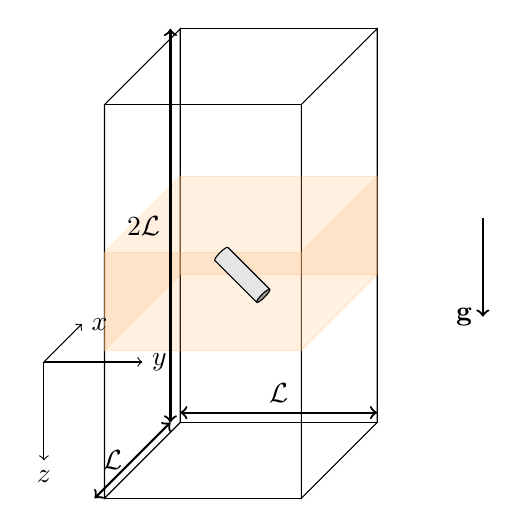
\begin{tikzpicture}[scale=2.5]

\def\opacity{0.8}



\draw (-0.5,-0.5,-0.5) -- ++(1,0,0) -- ++(0,2,0) -- ++(-1, 0, 0) -- cycle;
%\draw (-0.5,-0.5,-0.5) -- ++(1,0,0) -- ++(0,0,1) -- ++(-1, 0, 0) -- cycle;
\draw (-0.5,-0.5,-0.5) -- ++(0,2,0) -- ++(0,0,1) -- ++(0, -2, 0) -- cycle;
\draw[] (0.5,1.5,0.5) -- ++(-1,0,0) -- ++(0,-2,0) -- ++(1, 0, 0) -- cycle;
%\draw[] (0.5,0.5,0.5) -- ++(-1,0,0) -- ++(0,0,-1) -- ++(1, 0, 0) -- cycle;
\draw[] (0.5,1.5,0.5) -- ++(0,-2,0) -- ++(0,0,-1) -- ++(0, 2, 0) -- cycle;


\draw[orange!60, opacity=0.2 ,fill=orange!60, fill opacity=0.2](-0.5,0.25,-0.5) -- ++(1,0,0) -- ++(0,0.5,0) -- ++(-1, 0, 0) -- cycle;
\draw[orange!60, opacity=0.2 ,fill=orange!60, fill opacity=0.2](-0.5,0.25,-0.5) -- ++(0,0.5,0) -- ++(0,0,1) -- ++(0, -0.5, 0) -- cycle;
\draw[orange!60, opacity=0.2 ,fill=orange!60, fill opacity=0.2] (0.5,0.75,0.5) -- ++(-1,0,0) -- ++(0,-0.5,0) -- ++(1, 0, 0) -- cycle;
\draw[orange!60, opacity=0.2 ,fill=orange!60, fill opacity=0.2] (0.5,0.75,0.5) -- ++(0,-0.5,0) -- ++(0,0,-1) -- ++(0, 0.5, 0) -- cycle;



\node[cylinder, 
    draw = black, 
    text = black,
    cylinder uses custom fill, 
    cylinder body fill = black!10, 
    cylinder end fill = black!40,
    aspect = 0.2, 
    shape border rotate = 90, rotate =225, minimum height=0.8cm, minimum width=0.2cm] (c) at (0,0.45,0) {};

\draw[->, thick] (2.,1.5,2)--(2,1,2) node[left]{$\mathbf{g}$};

\draw[<->, thick] (-0.5,-0.45,-0.5)-- node[above]{$\mathcal{L}$} ++(1,0,0) ;
\draw[<->, thick] (-0.55,-0.5,-0.5) -- node[left]{$2\mathcal{L}$} ++(0,2,0);
%\draw[<->, thick] (0.5,1.55,0.5) -- node[above]{$12D$} ++(-1,0,0);
%\draw[<->, thick] (0.55,1.5,0.5) -- node[right,below]{$12D$} ++(0,0,-1);
\draw[<->, thick] (-0.55,-0.5,-0.5) -- node[left]{$\mathcal{L}$} ++(0,0,1);

%\draw[<->, thick,orange!90](0.55,0.75,0.5) -- node[right]{$6D$} ++(0,-0.5,0);
%\draw[<->, thick,orange!90](0.55,-0.5,0.5) -- node[right]{$8D$} ++(0,+0.75,0);
%\draw[<->, thick,orange!90](0.55,0.75,0.5) -- node[right]{$10D$} ++(0,+0.75,0);

%\draw (0.5,1.5,2) node[]{$\rho_f, \mu$};
\draw[->] (-1,0,0)--(-1,0,-0.5)node[right]{$x$};
\draw[->] (-1,0,0)--(-0.5,0,0)node[right]{$y$};
\draw[->] (-1,0,0)--(-1,-0.5,0)node[below]{$z$};


\end{tikzpicture}
\caption{Scheme of the computational domain (not to scale).}
\label{fig:domain}
\end{figure}
We explore the effect of $\chi$, $Ar$ and $\bar{\rho}$ within the range $\chi = \{2,4\}$, $Ar = \{24,96\}$ and $\bar{\rho} = \{1.5,10\}$. The cylinder is initiated with an angle $\phi =5 ^\circ$ and it is released at rest. In addition, a case with a larger density ratio was computed, starting at $\phi=60^\circ$, to investigate the damped oscillation regime. The computational domain for this problem is depicted in Figure \ref{fig:domain}. Its characteristic size length depends on the aspect ratio: for $\chi=2$, $\mathcal{L} = 12D$ while for $\chi=4$ $\mathcal{L} = 15D$. Note that the value prescribed for $\chi=2$ is larger than the one used in \citep{seyed2019}. We have checked that the present domain was sufficiently large by increasing its size of $25\%$ in all directions finding less than $2\%$ error on $\Omega L /U$ for the more challenging configuration ($Ar=24$, $\chi=4$). Obviously, larger domains might be used to avoid this small effect of the boundaries at the expense of a substantially larger numerical cost. However, we have to recall that the present paper is not aimed to provide domain size perfectly independent simulations of the problem but rather to provide bound to the quasi-steady assumptions. To this aim, we compare the numerical results to the model of section \ref{sec:scaling} which heavily relies on fit and also contains some error with respect to the simulation they are extracted from. Regarding the boundary conditions, the domain is biperiodic in the lateral directions while zero velocity and outflow conditions are imposed on the upstream and downstream boundaries, respectively. A uniform cell distribution is imposed in a rectangular region depicted in Figure \ref{fig:domain} as an orange volume. This region is located  $2D$ below the middle of the domain and extends up to $6D$ in the direction of gravity. In this flow region, $25$ cells are distributed per body diameter which is sufficient to accurately compute the dynamic for the range of Reynolds number investigated \citep{pierson2019}. The number of cells per mesh is 26 millions for $\chi=2$ and 46 millions for $\chi=4$. The time step is imposed such that the CFL always fall below $0.25$. To prevent the cylinder to exit the numerical domain the computational domain is moved in the vertical direction so as to keep the particle at least at a distance of $10D$ of the upstream boundary. More details on the domain translation technique can be found in \citet{rahmani2014,seyed2019} The magnitude of this domain translation is chosen to be the grid size ($D/25$). The simulations are run up until the cylindrical particle reaches its equilibrium position.


%Additionally, we have also computed a few cases with a larger density ratio starting with an angle $\phi=60^\circ$ to investigate the regime of damped oscillation. 




%The effects of $\chi$, $Ar$, and $\bar{\rho}$ on the behavior of a cylinder are explored within the ranges of $\chi = {2,4}$, $Ar = {24,96}$, and $\bar{\rho} = {1.5,10}$. The initial angle of the cylinder is set at $\phi =5 ^\circ$ and it is released at rest. In addition, cases with a larger density ratio are computed, starting at $\phi=60^\circ$, to investigate the damped oscillation regime. The computational domain is depicted in Figure \ref{fig:domain} and its characteristic size length depends on the aspect ratio. For $\chi=2$, $\mathcal{L} = 12D$, while for $\chi=4$, $\mathcal{L} = 15D$. Note that the value prescribed for $\chi=2$ is larger than the one used in a previous study (Seyed et al. 2019). The domain size was increased by $25\%$ in all directions to avoid any significant boundary effects, resulting in less than $3\%$ error on $\Omega L /U$ for the more challenging configuration ($Ar=24$, $\chi=4$). However, even larger domains could further reduce the boundary effects at the expense of a substantial numerical cost. The boundary conditions are biperiodic in the lateral directions, while zero velocity and outflow conditions are imposed on the upstream and downstream boundaries, respectively. A rectangular region with a uniform cell distribution is imposed below the middle of the domain, extending up to $6D$ in the direction of gravity, with 25 cells per body diameter. The number of cells per mesh is 26 million for $\chi=2$ and 46 million for $\chi=4$. The time step is chosen to ensure that the CFL number remains below $0.25$. To prevent the cylinder from exiting the numerical domain, the computational domain is moved vertically so that the particle remains at least $10D$ away from the upstream boundary. The simulations are run until the cylindrical particle reaches its equilibrium position. More details on the domain translation technique can be found in Rahmani et al. (2014) and Seyed et al. (2019). The purpose of this paper is not to provide a perfect simulation but to provide bounds to the quasi-steady assumptions by comparing the results with the model of Section \ref{sec:scaling}, which heavily relies on a fit with a few percent error with respect to the values obtained using direct numerical simulations.

%Larger domain might be of interesting to avoid any artificial confinement effects inherent to the slow decay of the disturbance at low Reynolds number \citep{fintzi2023}. However due to the important computational cost of the simulations we have prefered studying moderate Reynolds number ($Ar \gg 1$).

%In the present analysis one want to investigate the settling of moderately long cylinder. 






%particle at least a distance of l cr away from the inlet boundary
%The numerical domain is sketched in figure ... (not to scale)


%The computational
%domain along with different meshing zones are shown schematically in Fig. 1. As the cube moves, it
%would exit a domain with such a limited size fairly quickly. In order to circumvent this issue, we use
%a domain translation technique already discussed in Refs. [8,49,50], instead of using an extended
%domain in the vertical direction or a moving frame of reference. With this method, if the distance
%between the particle and the inlet boundary becomes smaller than a specified threshold (l cr = 6
%in our simulations), the computational domain is moved in the vertical direction so as to keep the
%particle at least a distance of l cr away from the inlet boundary. This is achieved by removing a
%certain number of grid layers from the outlet and adding the same number of layers to the inlet. The
%magnitude of this domain translation is chosen to be a multiple of the grid size (2x for all cases
%here) to avoid projection errors of the computed solution on the translated grid around the particle.
%The time step t is always kept smaller than 1 × 10 −3 for light cubes (m < 1) and smaller than
%2 × 10 −3 for dense cubes (m > 1). Most of our simulations are run up to at least t = 200, while in

%We start by revisiting the original Cox (1965) statement. 

%\section{Limit of validy for $Re_l \sim 1$}
%Were $\bm{U}$ and $\bm{\Omega}$ are the translating and rotating velocity of the particle, $m$ is the mass of the cylinder, $V$ its volume and $\bm{F}^h$ the hydrodynamic drag force.


%then, $\mathcal{A}$ is the added mass effect from translation, and $\mathcal{D}$ for rotation. 
%Besides, note that in this frame of reference the inertia tensor, $\bm{J}$, is function of time. 

%We keep the inertial term to quantity their relative importance as function of $Re$. 

%Dans le cas d'une particule solide dans l'air, il faut considerer l'inertie de la particule. Newsom et Bruce propose un modèle sympa mais attention il n'est qu'a l'ordre epsilon ... 

%\section{Deux limites distinctes}



%$ratio rho * Ar^2$ de l'ordre de 1.
%$Ar^2 << 1$ et on néglige le terme inertiel.

%Ou plutot particule chutant dand l'air (dans ce cas le terme inertiel est non négligeable meme pour les tout petit Re)
%Particule chutant dans un fluide, la le terme non inertiel devient négeigleable a petit Ar MAIS  plus grand Ar a priori non, et la masse ajoutée non plus.

\subsubsection{Numerical results}

%\paragraph{Ar=24}

%We start by investing the effect of moderate inertia by investigating the case $Ar=24$. The Reynolds number varies within the range $1.7 \leq Re \leq 1.9$ for $\chi=2$ and $2 \leq Re \leq 2.7$ for $\chi=4$.

To investigate the impact of moderate inertia on the rod motion we first consider the situation $Ar=24$. In this scenario, the Reynolds number will fluctuate between $1.7$ and $1.9$ when $\chi$ equals $2$, and between $2$ and $2.7$ when $\chi$ is $4$.

\begin{figure}[h]
\centering
\includegraphics[width=5cm]{U_z_phi_Ar24_chi2.pdf}
\includegraphics[width=5cm]{U_y_phi_Ar24_chi2.pdf}
\includegraphics[width=5cm]{Omega_Phi_Ar24_chi2.pdf}\\
\hspace{0.5cm}$(a)$ \hspace{4.5cm} $(b)$ \hspace{4.5cm} $(c)$\\
\includegraphics[width=5cm]{U_z_phi_Ar24_chi4.pdf}
\includegraphics[width=5cm]{U_y_phi_Ar24_chi4.pdf}
\includegraphics[width=5cm]{Omega_Phi_Ar24_chi4.pdf}\\
\hspace{0.5cm}$(d)$ \hspace{4.5cm} $(e)$ \hspace{4.5cm} $(f)$
\caption{Dimensionless sedimenting velocities for $Ar = 24$. $(a),$ $(d)$ : vertical sedimenting velocity, $(b)$, $(e)$ : drift velocity and $(c)$, $(f)$ : angular velocity. $-$ : direct numerical simulation results with $\bar{\rho} = 1.5$, $-\cdot-$: direct numerical simulation results with $\bar{\rho} = 10$, $--$ : prediction from equations \ref{eq:UpA**} - \ref{eq:OmegarA**} with $\bar{\rho} = 1.5$, $\cdot\cdot$ : prediction from equations \ref{eq:UpA**} - \ref{eq:OmegarA**} with $\bar{\rho} = 10$. Top panel corresponds to $\chi = 2$ and bottom panel to $\chi = 4$.}
\label{fig:DNS_Ar24}
\end{figure}

%For the shortest cylinder ($\chi=2$), one may observe a good agreement between the model made of equations \ref{eq:UpA**}, \ref{eq:UqA**} and \ref{eq:OmegarA**} and the direct numerical results (Figure \ref{fig:DNS_Ar24} (a), (b), (c)). Changing the density ratio from 1.5 to 10 have very little effect on the sedimenting velocities for this particular case. In the Figure \ref{fig:DNS_Ar24}, we also display the results for $\chi=4$. Although qualitative agreement is observed between the model and the numerical results the model overpredicts the drift velocity and the angular velocity. Also, for $\chi=4$ one may observe a stronger effect of particle inertia on the sedimenting velocities. In particular underdamped motion can be identified in this case. To further investigate this oscillating behvairour we have computed the settling of a rod with the same dimensionless parameters ($Ar=24$,$\chi = 4$) but with much larger density ratio ... Also to keep the computational tim reasonable the simulation starts with $\phi=60^\circ$.

For the shortest cylinder with aspect ratio $\chi=2$, there is a noticeable agreement between the results obtained from equations \ref{eq:UpA**} - \ref{eq:OmegarA**} (including particle inertia) and those from direct numerical simulations, as illustrated in Figure \ref{fig:DNS_Ar24} (a) - (c). Varying the density ratio from 1.5 to 10 has a negligible effect on the sedimentation velocities in this particular case. In Figure \ref{fig:DNS_Ar24} (d) - (f), we present the results for $\chi=4$. Although there is a qualitative agreement between the model and the numerical results, the model overestimates the drift velocity and the angular velocity. Moreover, for $\chi=4$, the effect of particle inertia on the sedimentation velocities is more pronounced. In particular, this case exhibits underdamped motion. To investigate this oscillating behavior further, we have carried out one simulation of the settling of a rod with the same dimensionless parameters ($Ar=24$, $\chi=4$), but with a much larger density ratio ($\bar{\rho}=50$). In order to maintain reasonable computational time, the simulation is initiated with $\phi=60^\circ$.
\begin{figure}[h]
\centering
\includegraphics[height=5cm]{Omega_Phi_rho50.pdf}
\includegraphics[height=5cm]{Phi_t_rho50.pdf}\\
\hspace{0.5cm}$(a)$ \hspace{5.5cm} $(b)$
\caption{Comparison between the simulation results and the quasi-steady model with $Ar=24$, $\chi=4$ and $\bar{\rho}=50$. (a) : Phase space diagram of the oscillator. (b) : Time evolution of the inclination angle. $-$ : direct numerical simulation results, $--$ : prediction from equations \ref{eq:UpA**} - \ref{eq:OmegarA**}. }
\label{fig:DNS_Ar24_rho50}
\end{figure}
There is a good agreement between the simulation and the model even if the model overpredicts the angular velocity (Figure \ref{fig:DNS_Ar24_rho50}). We recall that we neglect the history loads in equations \ref{eq:UpA**} - \ref{eq:OmegarA**} which may affect the initial transient since the rod starts from rest. One may also observe a good agreement between the oscillating period, the decrease in amplitude given by the numerical results and the model made of equations \ref{eq:UpA**} - \ref{eq:OmegarA**} (Figure \ref{fig:DNS_Ar24_rho50} (b)). This is somehow surprising since there is \textit{a priori} no reason for neglecting the history loads in the underdamped regime. They appear to have a negligible effect on this regime.


%\begin{figure}[h]
%\centering
%\includegraphics[width=5cm]{U_z_phi_Ar24_chi4_rho1_5.pdf}
%\includegraphics[width=5cm]{U_y_phi_Ar24_chi4_rho1_5.pdf}
%\includegraphics[width=5cm]{Omega_Phi_Ar24_chi4_rho1_5.pdf}
%\caption{Sedimenting velocities. $Ar = 24, \chi = 2$}
%\end{figure}

%\begin{figure}[h]
%\centering
%\includegraphics[width=5cm]{U_y_phi_Ar24_chi4_rho10.pdf}
%\includegraphics[width=5cm]{U_z_phi_Ar24_chi4_rho10.pdf}
%\includegraphics[width=5cm]{Omega_Phi_Ar24_chi4_rho10.pdf}
%\caption{$\bar{\rho}=10.,Ar = 24, \chi = 4$}
%\end{figure}

%\paragraph{Ar=96}


%We now consider much larger inertia effects ($Ar=96$). In this regime, the Reynolds number varies between $5.3$ and $6.2$ with $\chi = 2$, and between $5.8$ and $8.6$ with $\chi=4$. There is once again a good agreement between the quasi-steady model and the numeral results for $\chi=2$ (Figure \ref{fig:DNS_Ar96} (a)-(c)). This is quite unexpected due to the importance of inertia effects in this configuration. The agreement is less good for $\chi=4$ where the drift velocity and angular velocity (Figure \ref{fig:DNS_Ar96} (d)-(f)) are overestimated by the model. All the configuration lead to underdamped regimes, although it is much more pronounced for the highest aspect ratio and density ratio since for $\chi=2, \bar{\rho=1.5}$ the amplitude of the oscillation are very small and almost indistinguishable. We have also compared the oscillating period and the decrease in amplitude given by the numerical results and the model made of equations \ref{eq:UpA**}, \ref{eq:UqA**} and \ref{eq:OmegarA**} for the $Ar=96$, $\chi=4, \bar{\rho}=10$.

%In the present study, we investigate the influence of larger inertia effects ($Ar=96$) on the dynamics of a fluid-immersed cylinder. Within this regime, the Reynolds number is found to vary between $5.3$ and $6.2$ for $\chi=2$ and between $5.8$ and $8.6$ for $\chi=4$. Surprisingly, the quasi-steady model exhibits good agreement with numerical results for $\chi=2$ (as depicted in Figure \ref{fig:DNS_Ar96} (a)-(c)), despite the significant role played by inertia effects. However, for $\chi=4$, the model overestimates both the drift velocity and angular velocity (as shown in Figure \ref{fig:DNS_Ar96} (d)-(f)). We observe that all configurations result in underdamped regimes, with the highest aspect ratio and density ratio showing more pronounced effects. Moreover, for $\chi=2$ and $\bar{\rho}=1.5$, the amplitude of oscillation is considerably small and nearly indiscernible. Finally, we compare the numerical and model-based results (derived from Equations \ref{eq:UpA**}, \ref{eq:UqA**}, and \ref{eq:OmegarA**}) for $Ar=96$, $\chi=4$, and $\bar{\rho}=10$, by examining the oscillation period and the decay of amplitude.


\begin{figure}[h]
\centering
\includegraphics[width=5cm]{U_z_phi_Ar96_chi2.pdf}
\includegraphics[width=5cm]{U_y_phi_Ar96_chi2.pdf}
\includegraphics[width=5cm]{Omega_Phi_Ar96_chi2.pdf}\\
\hspace{0.5cm}$(a)$ \hspace{4.5cm} $(b)$ \hspace{4.5cm} $(c)$\\
\includegraphics[width=5cm]{U_z_phi_Ar96_chi4.pdf}
\includegraphics[width=5cm]{U_y_phi_Ar96_chi4.pdf}
\includegraphics[width=5cm]{Omega_Phi_Ar96_chi4.pdf}\\
\hspace{0.5cm}$(d)$ \hspace{4.5cm} $(e)$ \hspace{4.5cm} $(f)$
\caption{Dimensionless sedimenting velocities for $Ar = 96$. $(a),$ $(d)$ : vertical sedimenting velocity, $(b)$, $(e)$ : drift velocity and $(c)$, $(f)$ : angular velocity. $-$ : direct numerical simulation results with $\bar{\rho} = 1.5$, $-\cdot-$: direct numerical simulation results with $\bar{\rho} = 10$, $--$ : prediction from equations \ref{eq:UpA**} -\ref{eq:OmegarA**} with $\bar{\rho} = 1.5$, $\cdot\cdot$ : prediction from equations \ref{eq:UpA**}, \ref{eq:UqA**} and \ref{eq:OmegarA**} with $\bar{\rho} = 10$. Top panel corresponds to $\chi = 2$ and bottom panel to $\chi = 4$.}
\label{fig:DNS_Ar96}
\end{figure}

We now consider much larger inertia effects ($Ar=96$). Within this regime, the Reynolds number is found to vary between $5.3$ and $6.2$ for $\chi=2$ and between $5.8$ and $8.6$ for $\chi=4$. Surprisingly, the quasi-steady model exhibits good agreement with numerical results for $\chi=2$ (as depicted in Figure \ref{fig:DNS_Ar96} (a)-(c)), despite the significant role played by inertia effects. However, for $\chi=4$, the model overestimates both the drift velocity and angular velocity (as shown in Figure \ref{fig:DNS_Ar96} (d)-(f)). We observe that all configurations result in underdamped regimes. This regime is much more pronounced for $\chi=4$ and $\bar{\rho}=10$ than for $\chi=2$ and $\bar{\rho}=1.5$ for which the amplitude of oscillation is small and nearly indistinguishable. Finally, we compare the numerical and model-based results (derived from Equations \ref{eq:UpA**} - \ref{eq:OmegarA**}) for $Ar=96$, $\chi=4$, and $\bar{\rho}=10$, by examining the oscillation period and the decay of amplitude. The results are displayed on Figure \ref{fig:underdamped_Ar96}. The model slightly underpredicts the amplitude decay as well as the oscillation period. 




\begin{figure}[h]
\centering
\includegraphics[height=5cm]{Phi_t_Ar96_rho10}
\caption{Time evolution of the inclination angle ($Ar=96$, $\chi=4, \bar{\rho}=10$). $-$ : direct numerical simulation results, $--$ : prediction from equations \ref{eq:UpA**} - \ref{eq:OmegarA**}.}
\label{fig:underdamped_Ar96}
\end{figure}

\section{Discussion and conclusion}
\label{sec:discussion}

Based on the results presented above, two main conclusions can be drawn. Firstly, it can be inferred that the quasi-steady assumption holds true across a broad range of dimensionless parameters, as it is supported by both the experiments conducted by \citet{cabrera2022} and \citet{roy2019} and by the direct numerical simulations. Although these experiments and simulations do not strictly adhere to the condition $Ar \ll 1/\chi$, the quasi-steady assumption is still valid for a significantly larger range of values than initially predicted. This can be attributed to the magnitude of the angular velocity $\Omega$, which has the correct scaling but is at least three order of magnitude smaller than the anticipated value. As a result, $\Omega L / U \ll 1$ for all configurations except the highest inertial simulations (see Table \ref{tab:omega}). Aditionnally, these findings support the notion that the quasi-steady assumption remains valid as long as $\Omega L / U \ll 1$, thereby strengthening our analysis.

\begin{table}[h]
\centering
   \begin{tabular}{| l |c c| c c | c c c r |}
     \hline
      & \multicolumn{2}{l|}{\citet{cabrera2022}}  & \multicolumn{2}{c|}{\citet{roy2019}} & \multicolumn{4}{c|}{Direct numerical simulations}\\ 
      & \multicolumn{2}{c|}{$Ar \approx 0.147$}  & \multicolumn{2}{c|}{$Ar \approx 0.76$}  & \multicolumn{2}{c}{$Ar =24$} & \multicolumn{2}{c|}{$Ar = 96$}\\
      & $\chi=8$ & $\chi=16$ & $\chi=20$ & $\chi=100$ & $\chi=2$ & $\chi=4$ & $\chi=2$ & $\chi=4$\\\hline
     max$(\Omega _r L / |\mathbf{U}|)$ & 0.024 & 0.035 & 0.12 & 0.11 & 0.13 & 0.25 & 0.2 & 0.33\\ \hline
   \end{tabular}
\caption{Values of max$(\Omega _r L / |\mathbf{U}|)$ in the experiments of \citep{cabrera2022}, \citep{roy2019} and in the simulation results.}
\label{tab:omega}
 \end{table}

%Specifically, in the experiments conducted by \citet{cabrera2022}, the maximum value of ${\Omega L / U}$ is approximately 0.024 and 0.035 for $\chi=8$ and $\chi=16$, respectively. In the experiments conducted by \citet{roy2019}, the maximum value of ${\Omega L / U}$ is approximately 0.12 and 0.11 for $\chi=20$ and $\chi=100$, respectively. 

 

Secondly, it can be concluded based on the results of the previous section that particle inertia plays no significant role on the magnitude of the sedimenting velocities in the system under investigation. Hence, a correct estimate of $\Omega L / U$ can be obtained by disregarging the particle inertia in the equations of motion and considering the system made of equations \ref{eq:UpA**qs} - \ref{eq:OmegarA**qs}. We have solved this system for $\chi \in [2;500]$ and $Ar \in [0.001;150]$ by using the semi-empirical expression for the loads proposed by \citet{fintzi2023} for $\chi\leq 30$ and \citet{khayat1989} theory for $\chi > 30$. In each of the run we have computed the maximum value of $\Omega _r L / |\mathbf{U}|$ (Figure \ref{fig:OmegaLU}). 






%It even decreases  
%with ...

%We solve the non-linear system made of \ref{eq:UpA**}, \ref{eq:UqA**}, and \ref{eq:OmegarA**} neglecting the LHS. The results of this  For reason, which will appear clearer soon we investigate the results of sytem on a large range of $Ar$. 

%\begin{figure}[h]
%\centering
%\includegraphics[width=5cm]{Re_U.pdf}
%\includegraphics[width=5cm]{Re_Omega.pdf}
%\includegraphics[width=5cm]{Omega_L_U.pdf}\\
%\hspace{0.5cm}$(a)$ \hspace{5.5cm} $(b)$ \hspace{5.5cm} $(c)$
%\caption{Evolution of several quantities with $Ar$ or $\chi Ar$. $Re$, $Re_\Omega$ and $\Omega L/U$ are the maximum values encountered over the whole range of $\phi$. (a) : Reynolds number as function of $Ar$, (b) : Rotational Reynolds number as function of $Ar$ and (c) : $\Omega L/ U$ as function of $\chi Ar$.}
%\end{figure}

\begin{figure}[h]
\centering
\includegraphics[width=5cm]{Omega_L_U.pdf} \includegraphics[width=5cm]{Omega_L_U_KC.pdf}\\
\hspace{0.5cm}$(a)$ \hspace{5.5cm} $(b)$
\caption{Evolution of max($\Omega _r L/|\mathbf{U}|)$ with $\chi Ar$. Equations \ref{eq:UpA**qs} - \ref{eq:OmegarA**qs} are solved using a root-finding algorithm for 20 values of $\phi$ ranging between $0$ and $\pi/2$.}%$\Omega L/U$ are the maximum values encountered over the whole range of $\phi$.}
\label{fig:OmegaLU}
\end{figure}


For $Ar \chi \leq 10$ except for the smallest aspect ratio $\Omega L/ U $ scales as $Ar\chi$ in agreement with our scaling analysis. For larger $\chi Ar$ the rate of increase of $\Omega L/U$ decreases strongly, especially for $\chi \geq 12$. Indeeed it can be noted that qualitatively different behavior may be observed for moderate inertial effects ($Re_L\sim 1$) and very large aspect ratios ($\chi \gg 1$). \citet{fintzi2023} observed that for $\chi = 30$, the inertial torque scales as $T_i /(\mu U L^2) \sim Re_L^{1/3}$, yielding $T_i \sim \rho^{1/3} \mu^{2/3}U^{4/3}L^{7/3}$. By balancing this inertial torque with the resistive torque, we obtain $\Omega \sim \rho^{1/3}\mu^{-1/3}U^{4/3}L^{-2/3}$, and $\Omega L/U \sim Re_L^{1/3}$. Using the same scaling as in section \ref{sec:scaling} for the velocity, we obtain $\Omega L/U \sim Ar^{1/3}\chi^{1/3}$. Therefore, the rate of increase of $\Omega L/U$ is slower as the Reynolds number increases for elongated particle. This trend is even more pronounced for very long fibers (Figure \ref{fig:OmegaLU} (b)). In this regime, \citet{khayat1989} demonstrated that the inertial torque decreases with the Reynolds number for $Re_L \geq 4$. However, the validity of their theory for such high Reynolds numbers may be questionable, as their asymptotic solution requires $Re_L \ll \ln(\chi)$. Nonetheless, simulations performed by \citet{khair2018} and \citet{shin2006} indicate that the solutions proposed by \citet{khayat1989} remain valid for $Re_L \approx 10$ and $Re_L \approx 5$, respectively, for the longitudinal force on a long spheroid aligned with the flow direction and the torque on a long fiber, with $\chi = 100$. Moreover, \citet{khayat1989} models are in very good agreement with \citet{roy2019} experimental results for $\chi=100$ and $Re_L \approx 7.6$. Consequently, the solution provided by \citet{khayat1989} is considered to provide quantitatively accurate results up to $Re_L \approx 10$ as long as the fiber is adequately elongated ($\chi \geq 100$). If we consider that the quasi-steady assumption fails for values of $\Omega L/U$ larger than $0.2$, then we can expect the quasi-steady models to be accurate for $\chi Ar \approx 200$ if $\chi=2$, and for $\chi Ar \approx 40$ if $2 < \chi \leq 30$. However, for more elongated fibers, the quasi-steady assumption should remain valid as long as the underlying assumptions made in the derivation of \citet{khayat1989} models are fullfilled, particularly if $Re\ll 1$.


%In this paper particular attention was paid to discussing the range of parameters for which the underdamped regime is observed as well as its characteristic feature (oscillation period, rate of decrease of the amplitude) in comparison to simplified models. In particular, we have shown that the underdamped oscillator qualitatively reproduces the numerical results but not quantitatively. This may have significant consequences in atmospheric flows for which this solution is at the root of the observed particle orientation. A natural extension of this model might be to include the particle inertia in the parallel velocity equation which was neglected for the sake of simplicity. This will result in a third-order linear ordinary differential equation which may be easily solved. This model may be also used in practice to discuss rods wake instability such as the fluttering motion \citep{toupoint2019}. However, in such high inertial flow, there is no reason for the quasi-steady assumption to remain valid \citet{fabre2011}. Moreover, even under the quasi-steady limit, the loads on such bodies at high Reynolds numbers are only known for very few configurations \citep{pierson2019,kharrouba2021}.


This paper also focuses on the underdamped regime and its characteristics, such as oscillation period and amplitude decrease rate, in comparison to simplified models. It was found that the most simple model \textit{i. e.} the underdamped oscillator qualitatively reproduces numerical results but not quantitatively.  This may have significant implications for atmospheric flows where particle orientation is driven by this solution\citep{gustavsson2019,gustavsson2021}. To improve the model, particle inertia could be included in the parallel velocity equation, resulting in a third-order linear ordinary differential equation that can be easily solved. A natural perspective to this model might be to study rods wake instability, like fluttering motion \citep{toupoint2019}. However, in such high inertial flow, there is no reason for the quasi-steady assumption to remain valid \citet{fabre2011}. Moreover, even under the quasi-steady limit, the loads on such bodies at high Reynolds numbers are only known for very few configurations \citep{pierson2019,kharrouba2021}.

%However, this assumption may not be valid in high-inertia flows, and the loads on bodies at high Reynolds numbers are only known for a few configurations.




%one may anticipate the quasi-steady models to be valid for $\chi Ar \approx 200$ for $\chi=2$, $\chi Ar \approx 40$ for $2 <\chi \geq 30$. For more elongated fibre the quasi-steady assumption should remain valid as long as the assumption used for the derivation of \citet{khayat1989} results are respected (in particular $Re\ll 1$).


%If the quasi-steady assumption is invalid when $\Omega L/U$ exceeds 0.2, then we can expect the quasi-steady models to be accurate for $\chi Ar \approx 200$ if $\chi=2$, and for $\chi Ar \approx 40$ if $2 < \chi \geq 30$. However, for more elongated fibers, the quasi-steady assumption should remain valid as long as the assumptions made in the derivation of \citet{khayat1989} results are respected, particularly if $Re\ll 1$.


%L'un des premiers résultats majeurs est donc que les termes inertiels sot négligeables tant que $Re_D^2\ll 1$ ce qui est en fait assez peu restrictif. Oui mais attention on a toujours que $\Omega L/U$ doit etre petit pour negliger les couplages rotation translation plus les effets instationnaires. In practice the magnitude of this term can be readily obtained by computing the value of $Omega U^*$
%Also in the above set of equationn we have voluntary kept the  inertia term. Their magnitude will be discussed. discuter aussi de la mgnitude de tout cela en fonction du rapport de densité.



 %The Reynolds number based on the terminal velocity.
%The Reynolds number based on the sedimentation rate varies linearly with the Archimedes number for $Ar \ll 1$. For higher Archimedean numbers, the slope decreases. We can also observe the strong increase of the Reynolds number with $\chi$. Nevertheless this increase is less for $\chi \gg 1$ since in this limit the variation of the drag coefficient with $\chi$ is of the form $1/\ln\chi$ at the leading order.

%Dire que Reynolds scale bien avec Ar pour les bas Ar mais qu'ensuite la pente decroit. on peut s'attendre a un scaling en racine de Ar pour les grand Ar. Par aillerus on voit que pour chi grand Reynolds est peut depend de chi, en lien avec le fait que la dependan en chi est faible. Concernant Re omega, on voitt que l'no on a un comportement non monotone. Cela peut s'expliquer par le fait que pour chi grand le scaling pour le torque inertiel n'est pas le bon (reprendre mes notes.). Et cela explique le comportmene aussi non monotone en fonction de cui de Omega L /u (verifier ReOmega, car il ne semble pas se comporter lineairemeent aevc Ar au carré.)

%Ensuite faut il ajouter la meme chose pour les grands rapport de densité ?



%scipy.optimize.fsolve
%http://faculty.sfasu.edu/judsontw/ode/html-20180819/nonlinear03.html


%In the present analysis we have completely disregarded the unsteady effect execpt  


%parler de la solution temps court / des résultatst de Shin et al. qui montre que la solution quasi-statique est valable apres $l^2/\nu$ / tout cela versus solution quasi-statique. Oui mais c'est difficile detre plus precis que cela. En particulier quand commence la solution quasi-statique ? a partir de quel angle par exemple ?




%PERSPECTIVEs
%deriver la solution au temps court pour la chute dun spheroide.
%il faudrait aussi investiguer les regimes suivant ; Reynodls d'ordre 1 mais chi plus eleve. On pourrait par exemple utiliser de lAMR dans ce cas 
%Plus la solution au temps court a confirmer experimentalement.

%a terme il faudrait deriver la solution du troisieme ordre pour les oscillations (peut se faire avec la diagonalisation d'une matrice 3 3) + deriver la decroissance de la solution de Khayat et cox pour de stres grdn rapport d'aspect.

%par ailleurs il faudrait ajouter les oscillations du modele de K and C. Mais c'est bcp plus compliqué car le torque ne depends pas quadratiquement de UpUq et cela donne problamenet des equations bcp plus compliquées. C'est qqc a etudier, mais il faudrait pouvoir simuler de tres grand rapport d'aspect ... Basilisk ?

%parler du fluttering, mais a mon avis pas aller dans plus de details:
%- Ern et al. donne la freq d'oscillation mais les rapports de densité sont faibles
%- David propose un modele quasi-statique (comme nous). Est il valable ? diffiicle à dire il semble y avoir peu de résultats de fluttering dans le cas des grd rapport de densite ?
%- il y a pleins d'infos dans Ern et al. mais clairement c'est une etude à part entiere
%- on va s'aerreter la.

%Je pense que la conclusion de cela peut etre de dire que d'une part la lineratité des forces n'eest plus verifiee. Idem pour le torque. Donc deja le modele doit etre plus complique. Ensuite donner la vlaeur de $Omega L /U$ a laide des resultats de clement : le modele est il valabale ? de l'orde de 0.2. Donc a priori cela se tente. Oui sauf que dans ce raisonnement que choisi on a comme vitesse Uq ou Up. Si on choisi Up on a un ratio d'ordre 1. D'ailleurs cest quelque chose a discuter dans mon modele. Vu que le ratio Omega L/Up n'est pas forcement petit ... sauf dans la limite des tres bas nombre d'Archimede base sur Uq ...

% ensuite on a a priori des oscillations forcees


%Perspectives a long terme :
%- chute d'une spheroide includant les effets instationnaire. quel effet sur le regime des oscillations
%- fluttering
%- autre ?


\section{Acknowledgements}
ANR MUSCATs financial support is greatly appreciated. We thank Bernhard Mehlig for stimulating discussions and for pointing out the former studies on the underdamped oscillator. The author is indebted to Greg Voth for providing the experimental data of \citet{roy2019}. We also thank Jacques Magnaudet for fruitful discussions on the added mass torque.
%\section{Conclusion}

\appendix

%\include{added}
%\section{Added mass on a spheroid with small eccentricity}
\section{Added mass coefficients}
\label{app:added}
\begin{figure}[h!]
    \centering
        \includegraphics[height=0.22\textwidth]{A_x_d}
        \includegraphics[height=0.22\textwidth]{B_x_d}
        \includegraphics[height=0.22\textwidth]{Qx_d}
    \caption{Dimensionless added mass coefficients as a function of $\chi$. ($\blacksquare$) : \citet{loewenberg1993} results, $\bullet$ : present results based on JADIM code \citep{kharrouba2020}.}
    \label{fig:added}
\end{figure}
In this appendix, we compute the coefficient $A_p$, $A_q$ and $D_q$ by using the JADIM code for $ 1 \leq \chi \leq 15$. The numerical details concerning the code as well as the mesh properties can be found elsewhere \citep{kharrouba2020,kharrouba2021,pierson2021}. At the time $t=0$ we impose a constant linear or angular acceleration to a cylinder initially at rest. Since in the very short time limit viscous and rotational contributions are negligible in comparison to potential flow contribution \citep{mougin2002} one can easily recover the added mass coefficients by computing the loads on the body. Figures \ref{fig:added} display the dimensionless added mass coefficient $A_p^* = A_p / (\rho V), A_q^*= A_q / (\rho V)$ and $D_q^* = D_q/ (\rho VL^2)$ as a function of the aspect ratio. A good agreement is observed between the present results and \citet{loewenberg1993} results obtained using potential flow calculations. In the limit $\chi \gg 1$, $\chi A_p^*$ and $A_q^*$ tend toward a constant value. For the particular case $A_q^*$ this constant is simply $1$, $\textit{i.e.}$ the added mass coefficient on an infinitely long cylinder perpendicular to the flow direction. As a result, we propose the following correlation
%While the results for $A_p$ , $A_q$ are known (see ?), to he best of our knowledge the results for D q have not been published yet.

%The added mass tensors can be written as.
%The numerical framework is simple and can be found elsewhere \citep{auguste2010,kharrouba2020}.  





\begin{equation}
A_p^* = \frac{1}{\chi}\left(0.655-\frac{0.141}{1+\chi^{1.17}}\right),
\end{equation}
\begin{equation}
A_q^* = 1-\frac{0.828}{1+\chi^{1.12}}.
\end{equation}

To the best of our knowledge, the functional dependency of $D_q^*$ with respect to $\chi$ has not been published yet in the literature at least for $\chi \geq 1$. Figure \ref{fig:added} shows that in the limit $\chi \gg 1$ $D_q^*$ tends toward a constant value which is \textit{a priori} unknown. However, in the case of a Rankine ovoid, for $\chi \gg 1$, $D_q^*\approx 1/12$ \citet{howe2006}. Since in the limit of large aspect ratio one may assume that the rounded ends of the Rankine ovoid have little effect on the added mass coefficient, we propose the following empirical correlation  

%this coefficient can be computed in the case of a Rankine ovoid. in this case as $\chi \gg 1$ one have 

%To the best of our knowledge there is no formula for an infinitely long cylinder rotating. However 

% the added mass torque due to a unsteady rotaton of a cylinder. 



%The virtual mass of the cylinder is very close to one for chi=10. It tends to one as chi tends to infinity. On peut s'attendre a des effets non negligeables pour des rapport de densite de l'ordre de 1.

\begin{equation}
D_q^* = \frac{1}{12}-\frac{0.11}{(1+\chi^{0.8})},
\end{equation}
which matches closely the numerical results.







\section{Short-time asymptotic expansion}
\label{app:short}
We calculate the leading-order terms of the short-time asymptotic expansion. Since $\cos(\phi^{(0)}+\epsilon \phi^{(1)}) \sim \cos\phi^{(0)}-\epsilon \phi^{(1)}\sin\phi^{(0)}$ and $\sin(\phi^{(0)}+\epsilon \phi^{(1)}) \sim \sin\phi^{(0)}+\epsilon \phi^{(1)}\cos\phi^{(0)}$ at zero-th order equations \ref{eq:Upvd}, \ref{eq:Uqvd}, \ref{eq:Omegarvd} and \ref{eq:Phivd} simplifies to
\begin{align}
 \frac{d U_p ^{*(0)}}{dt^*}
    &= \mathcal{A}\cos \phi^{(0)},\\
\frac{d U_q ^{*(0)}}{dt^*}
    &= -\mathcal{B}\sin \phi^{(0)},\\
    \frac{d\Omega _r^{*(0)}}{dt^*}
    &= -\mathcal{C}U_p^{*(0)}U_q^{*(0)} ,\\
\frac{d \phi^{(0)}}{dt^*} &=0.
\end{align}
 The zero-th order solution is easily obtained and reads 
\begin{align}
%U_p ^{*(0)} &=  U_p^*(t^*=0) +  \left(\frac{\bar{\rho}-1}{\bar{\rho} + A_p^*}\right)t^*\cos \phi \\
%U_q ^{*(0)} &=  U_q^*(t^*=0) -  \left(\frac{\bar{\rho}-1}{\bar{\rho} + A_q^*}\right)t^*\sin \phi,\\
U_p ^{*(0)} &=   \mathcal{A}t^*\cos \phi^{(0)}, \\
U_q ^{*(0)} &=   -\mathcal{B}t^*\sin \phi^{(0)},\\
\Omega _r^{*(0)}
    &= \frac{\mathcal{A}\mathcal{B}\mathcal{C}}{3}t^{*3}\cos \phi^{(0)} \sin \phi^{(0)},\\
\phi^{(0)}&=\phi(t^*=0),
\end{align}
where we have assumed that the cylinder starts from rest. At first order equations \ref{eq:Upvd}, \ref{eq:Uqvd}, \ref{eq:Omegarvd} and \ref{eq:Phivd} give

\begin{align}
\frac{d U_p ^{*(1)}}{dt^*} 
    &= \frac{\mathcal{A}}{\mathcal{B}}\Omega _r ^{*(0)} U_q ^{*(0)}-\mathcal{A}\phi^{(1)}\sin\phi^{(0)}, \\
\frac{d U_q ^{*(1)}}{dt^*}    
    &=-\frac{\mathcal{B}}{\mathcal{A}}\Omega _r ^{*(0)} U_p ^{*(0)} - \mathcal{B}\phi^{(1)}\cos\phi^{(0)}, \\
%\begin{equation}
    \frac{d\Omega _r^{*(1)}}{dt^*}
    &= 0 ,\\
\frac{d \phi^{(1)}}{dt^*} &=\Omega _r^{*(0)}, 
\end{align}
which leads to
%\begin{align}
%\frac{d U_p ^{*(1)}}{dt^*} 
%    &= -\frac{5}{12}\mathcal{A}^2\mathcal{B}\mathcal{C}t^{*4}\cos \phi^{(0)} \sin ^2\phi^{(0)}, \\
%\frac{d U_q ^{*(1)}}{dt^*}    
%    &=- \frac{5}{12}\mathcal{A}\mathcal{B}^2\mathcal{C}t^{*4}\cos ^2\phi^{(0)} \sin \phi^{(0)}, \\
%\begin{equation}
%\Omega _r^{*(1)}
%    &= 0 ,\\
%\phi^{(1)}&=\frac{\mathcal{A}\mathcal{B}\mathcal{C}}{12}t^{*4}\cos \phi^{(0)} \sin \phi^{(0)}
%\end{align}
%then

\begin{align}
U_p ^{*(1)}
    &= -\frac{1}{12}\mathcal{A}^2\mathcal{B}\mathcal{C}t^{*5}\cos \phi^{(0)} \sin ^2\phi^{(0)}, \\
U_q ^{*(1)}    
    &=- \frac{1}{12}\mathcal{A}\mathcal{B}^2\mathcal{C}t^{*5}\cos ^2\phi^{(0)} \sin \phi^{(0)}, \\
%\begin{equation}
\Omega _r^{*(1)}
    &= 0,\\
\phi^{(1)}&=\frac{\mathcal{A}\mathcal{B}\mathcal{C}}{12}t^{*4}\cos \phi^{(0)} \sin \phi^{(0)}.
\end{align}

%\begin{align}
%    \frac{d\Omega _r^{*(2)}}{dt^*}
%    &= -\mathcal{C}U_p^{*(1)}U_q^{*(1)} ,\\
%\Omega _r^{*(2)}
%    &= -\frac{4}{9}\mathcal{A}^3\mathcal{B}^3\mathcal{C}^3t^{*11}\cos^3 \phi^{(0)} \sin ^3\phi^{(0)},\\
%\end{align}

\section{Quasi-steady loads}
\label{app:qsloads}
%\color{red} remplacer les reynolds par Re*.

%\color{black}

The expression of the quasi-steady loads used in this paper can be found below.

\subsection{Moderately long rods : $\chi \leq 30$}
\paragraph{Expression of $F_p$ : }
The expression of $F_p$ reads \citep{fintzi2023}
\begin{align}
F_p(Re_L^*,\chi,\theta) = -2\pi\mu |\mathbf{U}| L \cos \theta &\left(\frac{A_{Re=0}^{(1)}+A^{(1)}(Re_L^*)}{\ln(2\chi)}+\frac{A_{Re=0}^{(2)}+A^{(2)}(Re_L^*)}{\ln^2(2\chi)}+\frac{A_{Re=0}^{(3)}+A^{(3)}(Re_L^*)}{\ln^3(2\chi)} \right.\nonumber \\
    &\left. +\frac{A_{Re=0}^{(4)}+A^{(4)}(Re_L^*)}{\ln^4(2\chi)}+\frac{2.34}{\chi^{2/3}(\chi-\frac{1}{2})^{1.75}}\right),
    \label{eq:F_0all}
\end{align}
where $A_{Re=0}^{(1)} = 1$, $A_{Re=0}^{(2)} \approx 0.807$, $A_{Re=0}^{(3)} \approx 0.829$, $A_{Re=0}^{(4)} \approx 1.45$ \citep{kharrouba2021}. The first order inertial correction is null, $A^{(1)}(Re_L^*) = 0$ , while the second, third and fourth order inertial functions read
\begin{align}
    A^{(2)}(Re_L^*) &= \frac{1}{2}\left(\frac{E_1(2Re_L^*)+\ln(2Re_L^*)-e^{-2Re_L^*}+\gamma+1}{2Re_L^*}+E_1(2Re_L^*)+\ln(2Re_L^*)+\gamma-2 \right),\\
    A^{(3)}(Re_L^*) &= A_{A}^{(3)}(Re_L^*)+A_{B}^{(3)}(Re_L^*) +2A^{(2)}(Re_L^*)\ln{(2)},\\
    A^{(4)}(Re_L^*) &= 3\ln{(2)}\left(A_A^{(3)}(Re_L^*)+A_B^{(3)}(Re_L^*)\right) +3A^{(2)}(Re_L^*)\ln{(2)}^2   -0.636 Re_L^{*0.762},
\end{align}
where $\gamma$ is the Euler constant, $E_1(x) = \int_x^\infty \frac{e^{-t}}{t}dt$ the exponential integral function and here $Re_L^* = \rho |\mathbf{U}| L /(2\mu)$. One may observe that $|\mathbf{U}| \cos \theta = U_p$. 


\paragraph{Expression of $F_q$ : }

The expression of $F_q$ can be found in \citep{fintzi2023} and reads
\begin{align}
    F_q(Re_L^*,\chi,\theta) = 4\pi\mu |\mathbf{U}| L \sin \theta &\left(\frac{B_{Re=0}^{(1)}+B^{(1)}(Re_L^*)}{\ln(2\chi)}+\frac{B_{Re=0}^{(2)}+B^{(2)}(Re_L^*)}{\ln^2(2\chi)}+ \frac{ B_{Re=0}^{(3)}+B^{(3)}(Re_L^*)}{\ln^3(2\chi)} \right.\\
&+\left.\frac{B_{Re=0}^{(4)}+B^{(4)}(Re_L^*)}{\ln^4(2\chi)} -\frac{0.568}{\chi^{2/3}(\chi-\frac{1}{2})^{1.75}}\right).
    \label{eq:FAllchiT90ReFit}
\end{align}
where $B_{Re=0}^{(1)} = 1$, $B_{Re=0}^{(2)} \approx -0.193$, $B_{Re=0}^{(3)} \approx 0.214$, $B_{Re=0}^{(4)} \approx 0.387$ \citet{kharrouba2021}.
$B^{(1)}(Re_L^*) = 0$ and 
%To do so we make use of the theoretical terms derived by \citep{khayatInertiaEffectsMotion1989} namely,
\begin{align}
    B^{(2)}(Re_L^*) &= E_1\left(Re_L^*\right) +\ln{\left(Re_L^*\right)} - \frac{e^{-Re_L^*}-1}{Re_L^*} +\gamma-1\\,
    B^{(3)}(Re_L^*) &=  2\ln{(2)}B^{(2)}(Re_L^*) + B_e^{(3)}(Re_L^*),\\
    B^{(4)}(Re_L^*) &=  3\ln{(2)}^2B^{(2)}(Re_L^*) + 3 \ln{(2)} B_e^{(3)}(Re_L^*) + B_e^{(4)}(Re_L^*). 
\end{align} 
We have $|\mathbf{U}| \sin \theta = -U_q$.

\paragraph{Expression of $T_r^i$ : }
The expression of $T_r^i$ can be found in \citep{fintzi2023}
\begin{align}
    T_r^i(Re_L^*,\chi,\theta) = 
    \rho |\mathbf{U}|^2L^3\sin{(2\theta)}\frac{5\pi}{48(1+Re_L^{*1.991})^{0.331}}
    &\left(
        \frac{1}{\ln^2(3\chi)}
        +\frac{2.244 -1.813Re_L^{*0.543}}{\ln^3(3\chi)}
    \right.\\
    &\left.
        -\frac{3.603 + 8.854Re_L^{*0.538}}{\ln^4(3\chi)}
        -\frac{14.301(Re_L^*/\chi)^{0.448}}{\ln^5(3\chi)}
    \right) 
    \label{eq:torque_final}.
\end{align}
One may note that $|\mathbf{U}|^2\sin{(2\theta)} = -2U_pU_q$.
\paragraph{Expression of $T_r^\Omega$ : }

An expression for the resisting torque due to the particle rotation can be found in \citet{pierson2021} and may be expressed as
\begin{align}
T_r^\Omega=&-\frac{-\pi\mu\Omega _r L^3}{3}\left[\frac{1}{\ln(2\chi)}+\frac{1}{\ln^2(2\chi)}\left(\frac{11}{6}-\ln 2 + f(\chi,,Re_\Omega^*)\right)+\frac{1}{\ln^3(2\chi)}\left(\frac{161}{36}- \frac{\pi ^2}{12}-\frac{11}{3}\ln 2+(\ln 2)^2\right)\right. \nonumber\\
                             &\left. +\frac{1}{\ln^4(2\chi)}\left(1-\frac{1}{(2\chi)^{1.2}}\right)^5 \left(- \frac{5}{4}\zeta (3)+\frac{1033}{72}-\ln ^3 (2)+\frac{11}{2}\ln ^2(2) - \frac{161}{12}\ln 2-\pi ^2 \left(\frac{11}{24}-\frac{1}{4} \ln 2\right)\right)\right],
\label{eq:sl4_bism_re}
\end{align}
\noindent with $f(\chi,Re_\Omega^*) = 0.018\chi^{2.3}Re_\Omega^{*0.9}$ and $Re_\Omega^{*} = \rho |\boldsymbol{\Omega}| D^2 /\mu$.

%\color{blue} TO DO :
\subsection{Long rods : $\chi > 30$}
For sufficiently long rods \citet{khayat1989} expressions for the loads are accurate. In the following we present the \citet{khayat1989} expression still making use of the linearization proposed by \citep{lopez2017} for the forces. Also we make use of the $1/\ln\chi$ original expansion proposed by \citet{khayat1989} rather than the $1/\ln(2\chi)$ expansion.  % To the best of our knowledfe there was no proper validation of resiting torque on long fiber. Thus we will make use of the previous formula neglecting the inertial correction. Also we still make use of the linearization proposed by Guazzeli. Indeed the loads follow ... this accurately.

\paragraph{Expression of $F_p$ : }
\begin{equation}
F_p(Re_L^*,\chi,\theta) = \frac{-2\pi\mu |\mathbf{U}| L \cos \theta}{\ln\chi} \left(1-\frac{A^{(2)}(Re_L^*)-4\ln 2+3}{\ln\chi}\right)^{-1}.
\label{eq:F_pKC}
\end{equation}

\paragraph{Expression of $F_q$ : }
\begin{equation}
F_q(Re_L^*,\chi,\theta) = \frac{4\pi\mu |\mathbf{U}| L \sin \theta}{\ln\chi} \left(1-\frac{B^{(2)}(Re_L^*)+1/2-\ln 4}{\ln\chi}\right)^{-1}.
\label{eq:F_qKC}
\end{equation}

\paragraph{Expression of $T_r^i$ : }
%The expression of $T_r^i$ for lond rods can be found in \citep{khayat1989}
\begin{align}
    T_r^i(Re_L^*,\chi,\theta) = - \mu U L^2 \frac{\pi}{2}  \left(\frac{1}{\ln \chi}\right)^2 \left[\cos\theta \left(P(X) - Q(X) + P(Y) -Q(Y)\right) \right.\left.  + P(Y)- P(X)\right]\sin\theta
    \label{eq:torque_final},
\end{align}


with $Q(x) = \frac{E_1(x)+\ln(x)+\gamma}{x}$, $P(x) = \frac{2}{x}\left(1+\frac{e^{-x}-1}{x}\right)$, $X  = Re_L^* \left(1-\cos\theta\right)$ and $Y  = Re_L^* \left(1+\cos\theta\right)$.% and $Re_L  = \frac{1}{2} Re \chi$.
\paragraph{Expression of $T_r^\Omega$ : }
Since to the best of our knowledge there is no expression for this torque for finite inertia effect and very long fibers we make use of expression \ref{eq:sl4_bism_re} neglecting the inertial correction $f$.
%\color{black}





%\bibliographystyle{apalike-fr}
\bibliography{biblio}
\end{document}
